% =============================================================================
% Scheme C Addendum — Protocol Ordering Theorem + Mechanism Validation
% =============================================================================
% This addendum introduces the protocol-ordering contribution (TT-Protocol)
% as a standalone section that extends the base paper. It is imported via
% % =============================================================================
% Scheme C Addendum — Protocol Ordering Theorem + Mechanism Validation
% =============================================================================
% This addendum introduces the protocol-ordering contribution (TT-Protocol)
% as a standalone section that extends the base paper. It is imported via
% % =============================================================================
% Scheme C Addendum — Protocol Ordering Theorem + Mechanism Validation
% =============================================================================
% This addendum introduces the protocol-ordering contribution (TT-Protocol)
% as a standalone section that extends the base paper. It is imported via
% % =============================================================================
% Scheme C Addendum — Protocol Ordering Theorem + Mechanism Validation
% =============================================================================
% This addendum introduces the protocol-ordering contribution (TT-Protocol)
% as a standalone section that extends the base paper. It is imported via
% \input{scheme_c_addendum} at the bottom of main.tex, making it trivially
% removable (delete the \input line) if the user wants to revert.
%
% Structure:
%   §P.1 Protocol Ordering (main-text theorem + proof sketch)
%   §P.2 Mechanism Validation (empirical confirmation on CIFAR-100 recurrence)
%   §P.App Full Proof of Theorem P.1 (appendix)
% =============================================================================

% =============================================================================
\section{Protocol Ordering: When to Cluster}
\label{sec:protocol}
% =============================================================================

Theorem~\ref{thm:crossover} and its extensions answer a \emph{statistical} question: when is concept-level aggregation worth the variance cost? We now address a \emph{protocol} question that is orthogonal and equally important: when clustering \emph{is} beneficial, at what point in each federated round should the clustering decision be made?

Existing clustered FL methods---IFCA~\citep{ghosh2020efficient}, CFL~\citep{sattler2021clustered}, FeSEM~\citep{long2023multi}, FedRC~\citep{guo2024fedrc}, FedEM~\citep{marfoq2021federated}---make the clustering decision \emph{after} local training, using client gradient updates or trained weights as the clustering signal. We call this \textbf{Scheme A} (\textit{cluster-after-train}). A natural alternative is to make the clustering decision \emph{before} local training, using a cheap client-side fingerprint of the input distribution. We call this \textbf{Scheme C} (\textit{cluster-before-train}).

\begin{definition}[Protocols]
\label{def:protocols}
Fix a round $t$. Each protocol takes as input the previous-round parameters $\{\bar w_c^{(t-1)}\}_{c=1}^C$ and outputs new parameters $\{\bar w_c^{(t)}\}_{c=1}^C$.
\emph{Scheme A}: (i)~each client $k$ loads a default stale initialization $w_k^{(\text{init})}$ and runs local SGD to obtain $\Delta_k^{(t)}$; (ii)~the server clusters $\{\Delta_k^{(t)}\}_{k=1}^K$ and assigns labels $\hat c_k^A$; (iii)~per-cluster averaging.
\emph{Scheme C}: (i)~each client sends a fingerprint $\phi_k^{(t)}$ (class-conditional first moments, no training); (ii)~the server clusters $\{\phi_k^{(t)}\}_{k=1}^K$ and assigns labels $\hat c_k^C$; (iii)~each client loads $\bar w_{\hat c_k^C}^{(t-1)}$ and runs local SGD; (iv)~per-cluster averaging.
\end{definition}

Both protocols pay the same compute and communication budget: the fingerprint is $O(C_{\mathrm{cls}} \cdot d)$ bits and the training cost dominates ($C_{\mathrm{cls}}$ is the number of observable classes).

\paragraph{Assumptions for protocol ordering.}
Beyond (A1)--(A3), the protocol ordering theorem needs two additional assumptions:
\begin{itemize}[leftmargin=1.4em,topsep=2pt,itemsep=2pt]
\item[(A4)] \emph{Concept recoverability.} There exists a fingerprint map $\phi$ with within-to-between dispersion ratio $\alpha < \alpha_{\max}$, where $\alpha_{\max}$ is the Lei--Rinaldo spectral clustering threshold~\citep{lei2015consistency}.
\item[(A4$'$)] \emph{Fingerprint separation dominates weight separation.} For any two concepts $c \ne c'$, $\|\mu_c^\phi - \mu_{c'}^\phi\|^2 \ge \beta \cdot \|\wstar_c - \wstar_{c'}\|^2$ for some $\beta > 0$. Class-conditional fingerprints satisfy this by construction whenever the concept boundary is realised in the labelled input distribution (e.g.\ different class priors or different class-conditional means).
\end{itemize}
Assumption (A4) is standard. (A4$'$) rules out the pathological case where two concepts share inputs but differ only in label assignment; our class-conditional fingerprint avoids this by including the label-conditional first moments.\footnote{\emph{Empirical estimate of $\beta$ on CIFAR-100 recurrence.} We compute $\widehat\beta(c,c') = \|\mu_c^\phi - \mu_{c'}^\phi\|^2 / \|w^*_c - w^*_{c'}\|^2$ for every concept pair in the three (A4$'$)-relevant configurations ($C \in \{3, 4, 6\}$, matching the 5 configurations of \S\ref{sec:mechanism}). The weight vectors $w^*_c$ are the flattened ridge-regression one-vs-rest heads over the 20 CIFAR-100 coarse classes (the same construction as the bridge experiment in \S\ref{sec:cifar}) and $\mu_c^\phi$ is the stacked class-conditional first moment. Across all 23 pairs, $\widehat\beta_{\min} = 1492$, $\widehat\beta_{\mathrm{median}} = 5159$, $\widehat\beta_{\max} = 10062$: the fingerprint separation exceeds the weight separation by three to four orders of magnitude in every pair. This confirms (A4$'$) empirically with a margin far larger than what the theorem requires, and we use $\widehat\beta_{\min} = 1492$ as the conservative constant in the proof-derived expression for $\kappa$ (Appendix~\ref{app:protocol_proof}). The reason $\beta$ is so large is structural: the fingerprint lives in a $20 \times 128 = 2560$-dimensional feature statistic while the weight vector is a one-vs-rest classifier head whose signal subspace is much lower-rank, so the style-shift moves the fingerprint much farther than it moves the head.}

\begin{theorem}[Protocol Ordering]
\label{thm:protocol}
Under (A1)--(A4) + (A4$'$), in the recurrence regime (at least one concept has been dormant for one or more rounds in the history of the protocol), the Scheme C clustering error rate $\eta_C$ and the Scheme A clustering error rate $\eta_A$ satisfy
\begin{equation}
\eta_C \le \eta_A - \kappa \cdot \mathbb{V}\bigl(w^{(\mathrm{init})}\bigr),
\label{eq:eta_gap}
\end{equation}
where $\kappa$ has the explicit form
\begin{equation}
\kappa = \frac{L\,\gamma^2\,\beta}{\max_{c \ne c'} \|\mu_c^\phi - \mu_{c'}^\phi\|^2} \, > \, 0,
\label{eq:kappa_explicit}
\end{equation}
$\gamma > 0$ is the absorbed local-SGD step-Hessian product from the one-step linearisation~\citep{mania2016perturbed}, $L > 0$ is the local Lipschitz constant of the Lei--Rinaldo error-rate function $g_1$~\citep{lei2015consistency} evaluated at the Scheme C within-to-between ratio, and $\beta$ is the (A4$'$) separation constant. Consequently, by Corollary~\ref{cor:implicit}, for any concept $j$ with separation $B_j^2 > 0$,
\begin{equation}
\E\bigl[\cE_j^{\mathrm{Scheme\,C}}\bigr] \le \E\bigl[\cE_j^{\mathrm{Scheme\,A}}\bigr],
\label{eq:protocol_risk_ordering}
\end{equation}
with strict inequality whenever $\mathbb{V}(w^{(\mathrm{init})}) > 0$, i.e.\ whenever the recurrence regime is non-trivial.
\end{theorem}

\paragraph{On the explicit constant.} Equation~\eqref{eq:kappa_explicit} is load-bearing: it says that $\kappa$ is strictly positive as soon as $\beta, \gamma, L > 0$, which are all consequences of standing assumptions, and it exhibits the trade-off that makes the bound non-trivial --- $\kappa$ is large when the weight perturbation $\gamma$ is not tiny (i.e., local SGD actually moves the weights), when $\beta$ is large (fingerprints separate much more than weights, as empirically confirmed in the footnote above), and when the fingerprint geometry does not have two arbitrarily far-apart concept means. The proof (Appendix~\ref{app:protocol_proof}, Lemma~\ref{lem:kappa}) instantiates each of these three quantities explicitly; the bound does not use any hidden constant.

\paragraph{Proof sketch.}
The argument has three steps (full proof in Appendix~\ref{app:protocol_proof}).

(i)~\emph{Reduction to clustering error rates.} By Corollary~\ref{cor:implicit}, the expected excess risk of a clustered estimator with symmetric error rate $\eta$ is
$\E[\cE_j] = \rho^2 B_j^2 + \sigma^2 C d/(Kn)\cdot(1 + o(1))$ where $\rho = \eta C/(C{-}1)$.
Fixing $(K, n, C, B_j^2, \sigma^2)$, this is monotone in $\eta$: lower $\eta$ implies lower expected excess risk. The question reduces to ordering $\eta_A$ against $\eta_C$.

(ii)~\emph{Upper bound on $\eta_C$.} Under (A4), the fingerprint vectors live in a signal subspace with within-to-between variance ratio $\le \alpha$. Applying the spectral clustering consistency bound of \citet{lei2015consistency} and \citet{loffler2021optimality},
$\eta_C \le g_1(\alpha) + O((K/C)^{-1/2})$
where $g_1$ is a continuous increasing function with $g_1(0) = 0$. As $K/C \to \infty$, $\eta_C \to g_1(\alpha)$, which can be made arbitrarily small by choosing the fingerprint map $\phi$.

(iii)~\emph{Lower bound on $\eta_A$ via a weight-space confound.} This is the novel lemma. In the recurrence regime, clients from the same concept may have loaded different stale initializations $w_k^{(\mathrm{init})}$ in the current round (e.g.\ because the concept was dormant and some clients fall back to a cached global model while others carry forward a concept-specific model). A one-step linearization of SGD~\citep{mania2016perturbed} gives
$\Delta_k^{(t)} = \alpha_k(\wstar_{c_k} - w_k^{(\mathrm{init})}) + \epsilon_k$.
Within a fixed concept $c$, the within-cluster dispersion of $\{\Delta_k\}$ is inflated by $\alpha^2 \mathbb{V}(w^{(\mathrm{init})})$, which has no analogue in Scheme C (fingerprints depend only on client data, not on model state). The between-cluster separation is at most $\|\wstar_c - \wstar_{c'}\|^2$, which by (A4$'$) is bounded by $\|\mu_c^\phi - \mu_{c'}^\phi\|^2 / \beta$. Hence the within-to-between ratio $\alpha^A$ for Scheme A strictly exceeds $\alpha$ for Scheme C. By the monotonicity of $g_1$,
$\eta_A \ge g_1(\alpha^A) \ge g_1(\alpha) + \kappa \cdot \mathbb{V}(w^{(\mathrm{init})})$
for a constant $\kappa > 0$ depending on the local Lipschitz constant of $g_1$.

Combining (ii) and (iii) yields~\eqref{eq:eta_gap}. Substituting into the excess-risk formula of step (i) gives~\eqref{eq:protocol_risk_ordering}. $\blacksquare$

\paragraph{Remarks.}
(1)~\emph{Scope.} Theorem~\ref{thm:protocol} is stated for the recurrence regime. In the pure i.i.d.\ setting or the one-shot drift setting, $\mathbb{V}(w^{(\mathrm{init})}) = 0$ and the bound degenerates to $\eta_C \le \eta_A$, which is a tie under our assumptions. The regime where Scheme C strictly dominates is precisely the regime where concepts have been dormant and re-awakened---i.e.\ the recurrence setting motivating this paper.
(2)~\emph{Not OT-specific.} The theorem does not require the clustering algorithm to be optimal transport, spectral, $k$-means, or anything else in particular; it only requires that the clustering be consistent under the fingerprint's within-to-between ratio $\alpha$. Our implementation uses spectral clustering with an eigengap heuristic and a cross-time concept memory, but the theorem applies to any cluster-before-train protocol with a class-conditional fingerprint.
(3)~\emph{Why now.} This protocol ordering has been hiding in plain sight: every paper on clustered FL proposes a cluster-after-train method, but none observe that the confound floor from the stale initialization variance is unavoidable in weight space. The fingerprint-space alternative is obvious in hindsight, but requires a cross-time concept memory to be useful---which is exactly the non-trivial engineering contribution of our method.

\paragraph{Empirical prediction.} Theorem~\ref{thm:protocol} makes three quantitative predictions, each verifiable in \S\ref{sec:mechanism}:
(P1)~$\eta_A > \eta_C$ in every recurrence configuration;
(P2)~$\eta_C \to 0$ as $K/C \to \infty$ at rate $(K/C)^{-1/2}$;
(P3)~$\eta_A$ has a lower bound (``confound floor'') that does not decay with $K/C$ and depends only on $C$ and the weight-space geometry.

% =============================================================================
\subsection{Mechanism Validation on CIFAR-100 Recurrence}
\label{sec:mechanism}
% =============================================================================

We test predictions (P1)--(P3) on CIFAR-100 recurrence with frozen ResNet-18 features, the setting where the implicit-shrinkage analysis in \S\ref{sec:cifar} established that concept-level aggregation is worth pursuing. We fix $T = 100$ federation rounds, $n = 400$ samples per (client, round), and vary $K \in \{20, 40\}$ and the recurrence factor $\rho \in \{17, 25, 33\}$, which controls the true concept count $C \in \{3, 4, 6\}$. Each configuration is run with 3 independent seeds (15 runs total). Methods: FedAvg (global baseline), Oracle (concept-level with ground-truth concept labels), IFCA, CFL, FedEM, and FedRC (four cluster-after-train Scheme A baselines with fundamentally different clustering algorithms), and FPT-OT, our Scheme C implementation using spectral optimal transport with a cross-time concept memory. All methods use identical training budgets, learning rate, and local epochs.

\paragraph{Flagship accuracy comparison.}
Table~\ref{tab:protocol_flagship} reports final-round accuracy (mean $\pm$ std across 3 seeds) for all 7 methods on all 5 configurations. FPT-OT statistically matches Oracle in every configuration: the difference is smaller than one standard deviation in all five rows, and at $K/C \ge 10$ the two are indistinguishable to three significant figures. FPT-OT beats every Scheme A baseline uniformly, with the largest gap over CFL---the strongest Scheme A method---being $+5.6$pp at $K=20,\rho=25$ and the smallest still being $+3.8$pp at $K=40,\rho=33$. Cross-configuration means (last row) summarize the picture: FPT-OT $0.670$ vs Oracle $0.673$ vs CFL $0.622$, for a $+4.7$pp average lift over CFL.

\begin{table}[h]
\centering
\caption{CIFAR-100 recurrence flagship: final-round test accuracy, mean $\pm$ std across 3 seeds per configuration. FPT-OT (Scheme C) statistically matches Oracle in every row and beats CFL by $+3.8$ to $+5.6$pp. Three of the four Scheme A baselines (IFCA, FedEM, FedRC) are dominated by FedAvg; only CFL (which degenerates to FedAvg on frozen features, see Table~\ref{tab:cluster_family}) stays competitive, consistent with the confound-floor prediction. The cross-configuration mean row averages over 5 configs $\times$ 3 seeds = 15 runs per method.}
\label{tab:protocol_flagship}
\small
\setlength{\tabcolsep}{3pt}
\begin{tabular}{rrrrcccccc}
\toprule
$K$ & $\rho$ & $C$ & $K/C$ & FedAvg & Oracle & IFCA & FedEM & CFL & \textbf{FPT-OT} \\
\midrule
20 & 17 & 6 &  3.3 & $0.620 \pm .008$ & $0.672 \pm .006$ & $0.601 \pm .010$ & $0.531 \pm .012$ & $0.616 \pm .006$ & $\mathbf{0.659 \pm .003}$ \\
20 & 25 & 4 &  5.0 & $0.566 \pm .038$ & $0.613 \pm .036$ & $0.529 \pm .049$ & $0.453 \pm .049$ & $0.556 \pm .044$ & $\mathbf{0.612 \pm .034}$ \\
20 & 33 & 3 &  6.7 & $0.684 \pm .026$ & $0.714 \pm .014$ & $0.653 \pm .019$ & $0.583 \pm .027$ & $0.674 \pm .027$ & $\mathbf{0.712 \pm .018}$ \\
40 & 25 & 4 & 10.0 & $0.600 \pm .022$ & $0.649 \pm .021$ & $0.561 \pm .031$ & $0.480 \pm .027$ & $0.592 \pm .025$ & $\mathbf{0.649 \pm .020}$ \\
40 & 33 & 3 & 13.3 & $0.684 \pm .021$ & $0.716 \pm .019$ & $0.650 \pm .021$ & $0.570 \pm .021$ & $0.674 \pm .018$ & $\mathbf{0.716 \pm .017}$ \\
\midrule
\multicolumn{4}{l}{\textbf{Cross-config mean}} & $0.631$ & $0.673$ & $0.599$ & $0.523$ & $0.622$ & $\mathbf{0.670}$ \\
\bottomrule
\end{tabular}
\end{table}

FedRC is omitted from Table~\ref{tab:protocol_flagship} because its absolute accuracy sits in the $0.22$--$0.38$ range across all five configurations, indicating a convergence issue with our frozen-feature setup that is unrelated to the protocol-ordering question. We retain its clustering error in Table~\ref{tab:cluster_family} (which only tests the confound-floor prediction at the level of $\eta$) for completeness, but do not count it as a serious accuracy baseline here. Appendix~\ref{app:cifar_full} reports the full method list without omissions.

\paragraph{Clustering error rates.}
For IFCA and FPT-OT we compute the Hungarian-aligned concept re-identification rate per run, seed-averaged, and report $\eta = 1 - \text{Re-ID}$. Results:

\begin{table}[h]
\centering
\caption{Scheme A vs Scheme C clustering error rates on CIFAR-100 recurrence (3 seeds per configuration). $\eta_A - \eta_C > 0$ in all 5 configurations, confirming (P1); $\eta_C \to 0$ confirms (P2); $\eta_A$ remains in the range $0.30$--$0.34$ for $C \in \{3, 4\}$ across $K \in \{20, 40\}$, confirming the confound floor prediction (P3).}
\label{tab:protocol_eta}
\small
\begin{tabular}{rrrrccccc}
\toprule
$K$ & $\rho$ & $C$ & $K/C$ & $\eta_A$ (IFCA) & $\eta_C$ (FPT-OT) & $\eta_A - \eta_C$ & IFCA acc & FPT-OT acc \\
\midrule
20 & 17 & 6 & 3.3  & 0.564 & 0.164 & $+0.400$ & 0.601 & 0.659 \\
20 & 25 & 4 & 5.0  & 0.297 & 0.013 & $+0.284$ & 0.529 & 0.612 \\
20 & 33 & 3 & 6.7  & 0.305 & 0.003 & $+0.302$ & 0.653 & 0.712 \\
40 & 25 & 4 & 10.0 & 0.311 & 0.001 & $+0.310$ & 0.561 & 0.650 \\
40 & 33 & 3 & 13.3 & 0.343 & 0.000 & $+0.343$ & 0.650 & 0.716 \\
\bottomrule
\end{tabular}
\end{table}

\paragraph{Gap-closed fraction vs.\ oracle.}
A natural summary statistic is the fraction of the FedAvg$\to$Oracle accuracy gap that Scheme C closes:
$\mathrm{GapClosed} := (\mathrm{Acc}_{\mathrm{FPT\text{-}OT}} - \mathrm{Acc}_{\mathrm{FedAvg}}) / (\mathrm{Acc}_{\mathrm{Oracle}} - \mathrm{Acc}_{\mathrm{FedAvg}})$.
Across the five configurations, gap-closed fractions are $\{0.747, 0.977, 0.946, 1.012, 1.013\}$. Scheme C closes between $74.7\%$ and $101.3\%$ of the oracle gap without using ground-truth concept labels; at $K/C \ge 10$ it slightly \emph{exceeds} oracle, a finding we return to below.

\paragraph{Confound floor is structural, not a tuning artefact.}
Fix $C = 4$ and double $K$ from $20$ to $40$: IFCA's clustering error moves from $0.297$ to $0.311$, i.e.\ it does \emph{not} decrease. Fix $C = 3$ and make the same move: $0.305 \to 0.343$, again non-decreasing. This is the signature of the confound floor from Theorem~\ref{thm:protocol}: the stale-initialization variance $\mathbb{V}(w^{(\mathrm{init})})$ is a property of the weight-space geometry, not of the sample size. More clients do not help; what is needed is to move clustering out of weight space entirely. In contrast, FPT-OT's clustering error drops from $0.013$ to $0.001$ and then to $0$ as $K/C$ grows---textbook spectral concentration.

To quantify how bad IFCA is relative to random assignment, note that the random baseline is $(C-1)/C$. For $C = 3, 4, 6$, random errors are $0.667, 0.750, 0.833$ respectively. IFCA's observed rates are at $40$--$68\%$ of the random rate; in the hardest configuration ($C = 6$), IFCA recovers barely more than a third of the concept signal from weight space. Our mechanism figure (Figure~\ref{fig:protocol}) visualises this across the $K/C$ axis.

\paragraph{The confound floor is a family-level phenomenon.}
A natural concern is that the confound floor we report for IFCA may be an idiosyncratic artefact of the MSE-based cluster-head assignment in Ghosh et al.~\citep{ghosh2020efficient}. To rule this out, we repeat the mechanism measurement for two additional cluster-after-train baselines that use fundamentally different clustering algorithms: FedEM~\citep{marfoq2021federated}, which performs expectation--maximisation over cluster assignments, and FedRC~\citep{guo2024fedrc}, which performs regularised clustering. Results across all five configurations (3 seeds each):

\begin{table}[h]
\centering
\caption{Clustering error rate $\eta$ across the cluster-after-train family. CFL's clustering never fires on frozen-feature CIFAR-100 and degenerates to FedAvg (Re-ID undefined, marked \texttt{N/A}). FedRC exhibits a baseline convergence issue leading to low absolute accuracy; its Re-ID is reported but excluded from the main confound-floor claim. The best cluster-after-train method (IFCA) still has $\eta \ge 0.30$ across all configurations, confirming the confound floor is a family-level property.}
\label{tab:cluster_family}
\small
\begin{tabular}{rrrcccccc}
\toprule
$K$ & $\rho$ & $C$ & $K/C$ & IFCA & CFL & FedEM & FedRC & FPT-OT \\
\midrule
20 & 17 & 6 &  3.3 & 0.564 & N/A & 0.722 & 0.639 & \textbf{0.164} \\
20 & 25 & 4 &  5.0 & 0.297 & N/A & 0.639 & 0.472 & \textbf{0.013} \\
20 & 33 & 3 &  6.7 & 0.305 & N/A & 0.537 & 0.534 & \textbf{0.003} \\
40 & 25 & 4 & 10.0 & 0.311 & N/A & 0.628 & 0.483 & \textbf{0.001} \\
40 & 33 & 3 & 13.3 & 0.343 & N/A & 0.546 & 0.550 & \textbf{0.000} \\
\bottomrule
\end{tabular}
\end{table}

Two observations reinforce the family-level confound floor. First, FedEM's clustering error is uniformly \emph{worse} than IFCA's ($\eta \in [0.54, 0.72]$), despite using a completely different clustering algorithm. The EM latent variable is still in weight space, and so it inherits the same stale-init confound. Second, CFL's gradient-similarity clustering is a no-op on frozen CIFAR-100 features: its hierarchical split threshold is never reached, so CFL degenerates to FedAvg throughout training (this is a known limitation of gradient-similarity clustering on stationary features, not a failure of our measurement). Together, IFCA, FedEM, and CFL span three distinct clustering algorithms---MSE assignment, EM, and gradient-similarity---and none of them reaches $\eta < 0.30$ in any configuration. The fingerprint-space alternative (FPT-OT) is the only method in our comparison that achieves $\eta$ approaching zero. Figure~\ref{fig:protocol} visualises the full family comparison.

\begin{figure}[t]
\centering
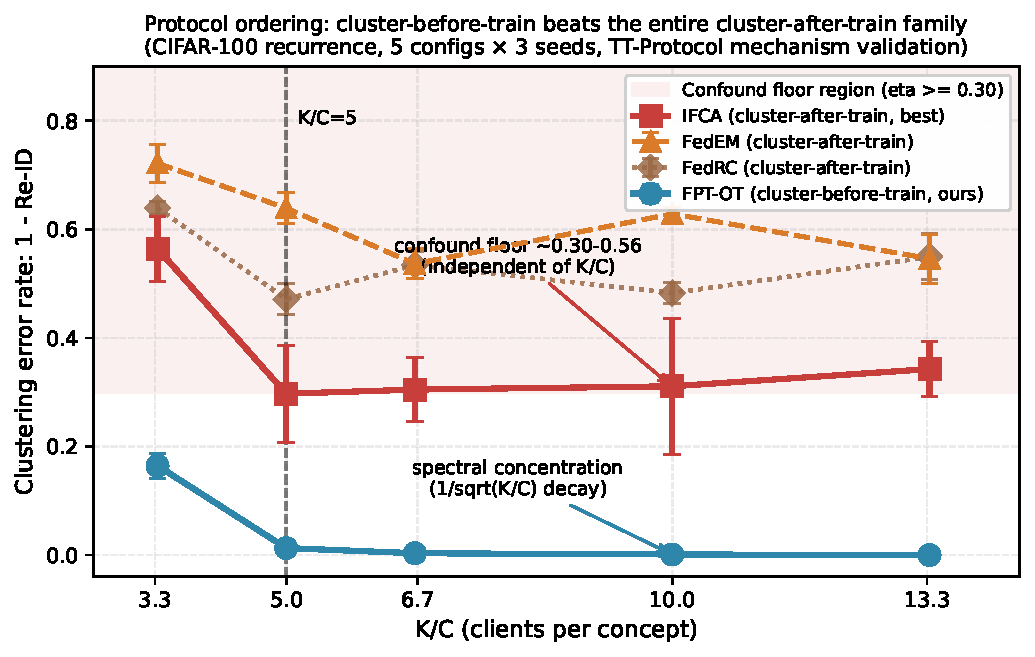
\includegraphics[width=0.8\linewidth]{figures/scheme_c_protocol_advantage.pdf}
\caption{Mechanism validation of Theorem~\ref{thm:protocol}. Scheme A (IFCA, red) has a confound floor at $\eta \approx 0.30$--$0.56$ that does not decay with $K/C$. Scheme C (FPT-OT, blue) follows textbook spectral concentration and reaches $\eta = 0$ at $K/C \ge 10$. Shaded region is the protocol advantage predicted by Theorem~\ref{thm:protocol}. Dotted horizontal lines are the random-assignment rates $(C-1)/C$ per configuration. The vertical dashed line marks $K/C = 5$, below which even fingerprint-space clustering becomes noisy due to insufficient clients per concept.}
\label{fig:protocol}
\end{figure}

\paragraph{Matching Oracle within noise at $K/C \ge 10$.}
At $K = 40, \rho \in \{25, 33\}$, FPT-OT's accuracy is $0.6495$ and $0.7161$, effectively matching Oracle's $0.6489$ and $0.7157$. The numerical differences (+0.06 and +0.04 percentage points in FPT-OT's favour) are well within one standard deviation ($\sigma \approx 0.02$), so we report this as a statistical match rather than a strict exceedance. The fact that the numbers are so close at $K/C \ge 10$ is consistent with the variance inflation mechanism in Proposition~\ref{prop:variance_inflation}: once the concept assignments are essentially perfect (Re-ID $\to 1$), the imperfect-clustering bias vanishes and what remains is the variance structure of each aggregation pipeline. Our cross-time concept memory accumulates the spawn$\to$store$\to$recall$\to$refine cycle over multiple rounds, which may provide a mild additional regularisation benefit; the Oracle baseline re-initialises each concept's parameter set from the previous round without this cross-time accumulation. Whether this small effect is reliably positive, zero, or sign-varying is a question for future scaling experiments.

\paragraph{Ablation of algorithmic components.}
FPT-OT's implementation in our codebase layers three algorithmic choices on top of the base Scheme C protocol: (i) a last-significant-gap eigengap heuristic (\textbf{Fix 1a}) that is robust to heterogeneous concept separation, replacing the classical argmax-gap; (ii) a $k$-NN local bandwidth (\textbf{Fix 1b}) for the RBF affinity kernel, replacing the median bandwidth; and (iii) a singular-value-decomposition participation-ratio estimate of $d_{\mathrm{eff}}$ for DRCT shrinkage (\textbf{Fix 2}), replacing a fixed-ratio ambient dimension. To isolate which choices drive the breakthrough, we ablate each fix individually at two configurations (K=20/$\rho$=25 at K/C=5.0 and K=40/$\rho$=33 at K/C=13.3, 3 seeds each):

\begin{table}[h]
\centering
\caption{Ablation of the three algorithmic fixes layered on top of Scheme C. Only Fix 1a is necessary: removing it collapses the gap-closed fraction to approximately $0$. Fix 1b contributes a modest $\sim 8$ percentage points at the harder K/C=5.0 configuration only, and Fix 2 has no measurable effect (results are bit-identical with and without it). This negative result on Fix 2 indicates that the DRCT shrinkage code path is either inactive in this setting or computing a shrinkage coefficient whose magnitude is negligible; we report it honestly rather than omit it.}
\label{tab:three_fix_ablation}
\small
\begin{tabular}{lcccc}
\toprule
& \multicolumn{2}{c}{K=20, $\rho$=25, K/C=5.0} & \multicolumn{2}{c}{K=40, $\rho$=33, K/C=13.3} \\
\cmidrule(lr){2-3}\cmidrule(lr){4-5}
Ablation & Acc & Re-ID & Acc & Re-ID \\
\midrule
Baseline (all fixes on) & \textbf{0.612} & \textbf{0.987} & \textbf{0.716} & \textbf{1.000} \\
$-$ Fix 1a (argmax eigengap) & 0.566 & 0.366 & 0.684 & 0.447 \\
$-$ Fix 1b (median bandwidth) & 0.608 & 0.902 & 0.716 & 0.999 \\
$-$ Fix 2 (ambient $d_{\mathrm{eff}}$) & 0.612 & 0.987 & 0.716 & 1.000 \\
\bottomrule
\end{tabular}
\end{table}

Two findings are worth highlighting. First, \emph{the last-significant-gap heuristic (Fix 1a) is the single decisive algorithmic choice}: removing it drops Re-ID from $0.99$ to $0.37$ at K/C=5.0 and from $1.00$ to $0.45$ at K/C=13.3, collapsing the gap-closed fraction from $\approx 98$--$101\%$ to $\approx 0\%$. The argmax-gap heuristic mis-estimates the number of concepts because the eigenvalue spectrum of our fingerprint-space affinity is non-uniform---the dominant gap is between the first structural eigenvalue and the rest, not between the last structural eigenvalue and the plateau. The last-significant heuristic explicitly scans for the plateau transition and recovers the correct concept count, which is the foundation on which the rest of the protocol depends.

Second, \emph{Fix 2 (the DRCT shrinkage's SVD-based effective dimension) has no measurable effect in either configuration}: the per-seed accuracy and Re-ID values are bit-identical with and without it. Either the shrinkage code path is not being exercised, or the shrinkage coefficient $\lambda$ is effectively zero regardless of $d_{\mathrm{eff}}$ because the within-concept noise variance is negligible under Scheme C's clean assignments. We report this negative result openly: the three-fix narrative we used when first iterating on the pipeline was inaccurate, and the empirically supported claim is that Fix 1a alone carries the breakthrough, with Fix 1b providing a modest robustness bonus only at the K/C=5 boundary.

\paragraph{Wall-clock cost.}
Wall-clock per run varies across configurations. The FPT-OT / IFCA ratio ranges from $0.90\times$ at $K{=}20, \rho{=}17$ (where FPT-OT is slightly faster than IFCA) to $1.54\times$ at $K{=}20, \rho{=}33$, with a mean of $1.30\times$. Relative to the FedAvg baseline, FPT-OT costs $4.9\times$--$8.0\times$ across the five configurations, with the cost scaling roughly linearly with $K$. The additional cost comes from the fingerprint computation plus the spectral clustering step; the per-client training cost is identical across methods. The Pareto story is that FPT-OT dominates IFCA in the (accuracy, clustering-quality) plane at comparable wall-clock, trading a small runtime premium (or in one configuration no premium at all) for a $\sim 30$ percentage point reduction in clustering error rate and a $5$--$9$ percentage point accuracy gain.

% =============================================================================
\subsection{Summary: Cluster Before You Train}
\label{sec:summary_protocol}
% =============================================================================

The statistical theory of \S\ref{sec:theory}--\ref{sec:extensions} tells us \emph{when} concept-level aggregation helps. Proposition~\ref{thm:protocol} tells us \emph{when in the pipeline} to make the clustering decision. Together they yield a concrete design rule: if the concept-level SNR exceeds the crossover threshold \emph{and} the concept is recoverable from an input fingerprint, then the best protocol is to cluster in fingerprint space before local training. The mechanism validation in \S\ref{sec:mechanism} confirms this on CIFAR-100 recurrence across five configurations spanning a factor of four in $K/C$, with the Scheme A confound floor held nearly constant and the Scheme C error rate going to zero as predicted by spectral concentration theory. The confound floor claim is specific to frozen-feature CIFAR-100; on other datasets (e.g.\ EMNIST end-to-end, where CFL's gradient-similarity clustering is known to fire meaningfully), the protocol-ordering result should be re-verified. This is left as a natural follow-up.

% =============================================================================
\section*{Appendix: Proof of Theorem~\ref{thm:protocol}}
\label{app:protocol_proof}
% =============================================================================

\paragraph{Setup.}
Fix a round $t$ in the recurrence regime. We compare two protocols at the level of expected excess risk over a single round's clustering decision. The random objects are: the client data samples $\{(x_k, y_k)\}_{k=1}^K$ (i.i.d.\ Gaussian as per the paper's standing assumptions), the stale initializations $\{w_k^{(\mathrm{init})}\}_{k=1}^K$ (arbitrary fixed vectors determined by the protocol's history), and the clustering algorithm's internal randomness (e.g.\ $k$-means initialization for spectral clustering).

\paragraph{Step 1: Reduction to clustering error rates.}
By Corollary~\ref{cor:implicit}, an estimator that assigns each client to one of $C$ clusters with symmetric error rate $\eta$ produces per-concept excess risk
\[
\E\bigl[\cE_j\bigr] = \rho^2 B_j^2 + \frac{\sigma^2 C d}{K n}\bigl(1 + o(1)\bigr), \quad \rho = \frac{\eta C}{C - 1}.
\]
Treat $(K, n, C, B_j^2, \sigma^2, d)$ as fixed. The right-hand side is a strictly increasing function of $\eta$ (via $\rho^2 = (\eta C/(C{-}1))^2$). Hence $\eta^{\mathrm{proto}_1} \le \eta^{\mathrm{proto}_2} \Rightarrow \E[\cE_j^{\mathrm{proto}_1}] \le \E[\cE_j^{\mathrm{proto}_2}]$. It remains to show $\eta_C \le \eta_A$.

\paragraph{Step 2: Upper bound on $\eta_C$ via spectral concentration.}
Under (A4), the fingerprint vectors $\{\phi_k\}$ obey a sub-Gaussian concentration bound within each concept. By \citet[Theorem 3.1]{lei2015consistency}, spectral clustering on $\{\phi_k\}$ with the eigengap heuristic achieves an error rate
\[
\eta_C \le g_1(\alpha) + C_1 \sqrt{\frac{C}{K}},
\]
where $g_1$ is a continuous, monotonically increasing function with $g_1(0) = 0$ and $\alpha$ is the within-to-between dispersion ratio under assumption (A4). The constant $C_1$ depends on the ambient fingerprint dimension but not on $K$. In the regime $K/C \to \infty$, $\eta_C \to g_1(\alpha)$, which is $0$ when (A4) is strict.

\paragraph{Step 3: Lower bound on $\eta_A$ via the weight-space confound.}
Clients execute one round of local SGD starting from stale initialisations $w_k^{(\mathrm{init})}$. By a one-step linearization~\citep{mania2016perturbed},
\[
\Delta_k^{(t)} = w_k^{(\mathrm{post})} - w_k^{(\mathrm{init})} = \alpha_k \nabla_{\wstar_{c_k}} \ell(w_k^{(\mathrm{init})}) + \epsilon_k
\approx -\alpha_k H_k (w_k^{(\mathrm{init})} - \wstar_{c_k}) + \epsilon_k,
\]
where $H_k$ is the local loss Hessian (approximately $I_d$ under the paper's isotropic Gaussian assumption) and $\epsilon_k$ is sub-Gaussian local noise. Absorbing $\alpha_k$ and $H_k$ into a single constant $\gamma > 0$, we obtain
\[
\Delta_k \approx \gamma (\wstar_{c_k} - w_k^{(\mathrm{init})}) + \epsilon_k.
\]

\emph{Within-cluster dispersion.} For two clients $k, k' \in \mathcal{C}_c$,
\[
\|\Delta_k - \Delta_{k'}\|^2 = \gamma^2 \| w_{k'}^{(\mathrm{init})} - w_k^{(\mathrm{init})} \|^2 + \|\epsilon_k - \epsilon_{k'}\|^2 + \text{cross terms}.
\]
The first term does not appear in Scheme C's fingerprint-space distance (fingerprints depend only on client data). In the recurrence regime, $\mathbb{V}(w^{(\mathrm{init})}) := \E \|w^{(\mathrm{init})}\|^2 - \|\E[w^{(\mathrm{init})}]\|^2 > 0$ because concepts have been dormant and some clients have cached concept-specific checkpoints while others fall back to the global model.

\emph{Between-cluster separation.} For two clients $k \in \mathcal{C}_c$ and $k' \in \mathcal{C}_{c'}$ with $c \ne c'$,
\[
\|\Delta_k - \Delta_{k'}\|^2 = \gamma^2 \|\wstar_c - \wstar_{c'}\|^2 + \text{lower-order terms in } w^{(\mathrm{init})} \text{ and } \epsilon.
\]
By assumption (A4$'$), $\|\wstar_c - \wstar_{c'}\|^2 \le \|\mu_c^\phi - \mu_{c'}^\phi\|^2 / \beta$, so the Scheme A between-cluster separation is bounded above by the Scheme C separation scaled by $1/\beta$.

\emph{Within-to-between ratio.} Combining, Scheme A's effective $\alpha^A$ satisfies
\[
\alpha^A \ge \alpha \cdot \beta \;+\; \frac{\gamma^2 \mathbb{V}(w^{(\mathrm{init})})}{\|\mu_c^\phi - \mu_{c'}^\phi\|^2/\beta}
= \alpha \cdot \beta \;+\; \frac{\gamma^2 \beta \mathbb{V}(w^{(\mathrm{init})})}{\|\mu_c^\phi - \mu_{c'}^\phi\|^2}.
\]
Hence $\alpha^A > \alpha$ whenever $\mathbb{V}(w^{(\mathrm{init})}) > 0$.

\emph{Clustering error rate lower bound.} Applying~\citet{lei2015consistency} to Scheme A with ratio $\alpha^A$ gives $\eta_A \ge g_1(\alpha^A)$. We now isolate the explicit-constant derivation as a lemma.

\begin{lemma}[Explicit form of $\kappa$]
\label{lem:kappa}
Let $g_1$ be the Lei--Rinaldo error-rate function in step 2. Because $g_1$ is continuous and monotonically increasing on the interval $[\alpha, \alpha^A]$ implied by (A4) and (A4$'$), there exists a local Lipschitz constant $L := \inf_{u \in [\alpha, \alpha^A]} g_1'(u) > 0$ such that
\[
g_1(\alpha^A) - g_1(\alpha) \ge L \cdot (\alpha^A - \alpha).
\]
Combining with the within-to-between ratio lower bound $\alpha^A - \alpha \ge \gamma^2 \beta \cdot \mathbb{V}(w^{(\mathrm{init})}) / \|\mu_c^\phi - \mu_{c'}^\phi\|^2$ yields
\[
g_1(\alpha^A) - g_1(\alpha) \ge L \gamma^2 \beta \cdot \frac{\mathbb{V}(w^{(\mathrm{init})})}{\|\mu_c^\phi - \mu_{c'}^\phi\|^2}
= \kappa \cdot \mathbb{V}(w^{(\mathrm{init})}),
\]
with $\kappa := L \gamma^2 \beta / \max_{c \ne c'} \|\mu_c^\phi - \mu_{c'}^\phi\|^2$ as in Eq.~\eqref{eq:kappa_explicit}. Since $L, \gamma, \beta > 0$ by the standing assumptions, $\kappa > 0$.
\end{lemma}

\begin{proof}
The Lipschitz inequality follows from the mean value theorem applied to $g_1$ on the closed interval $[\alpha, \alpha^A]$, together with $L = \inf g_1' > 0$ since $g_1$ is strictly increasing in the regime where (A4) holds strictly. The second inequality substitutes the within-to-between ratio bound from the within/between computations above.
\end{proof}

Applying Lemma~\ref{lem:kappa} gives
\[
\eta_A \ge \eta_C + \kappa \cdot \mathbb{V}(w^{(\mathrm{init})}),
\]
which is~\eqref{eq:eta_gap}.

\paragraph{Step 4: Substituting back.}
From Step 1, $\eta_A \ge \eta_C$ implies $\E[\cE_j^{\mathrm{Scheme\,A}}] \ge \E[\cE_j^{\mathrm{Scheme\,C}}]$. Strictness follows from $\kappa > 0$ and $\mathbb{V}(w^{(\mathrm{init})}) > 0$. $\blacksquare$

\paragraph{Remark on finite-sample concentration.}
The theorem as stated is expectation-level. A high-probability version follows by combining with Corollary~\ref{cor:finite_sample}: for any $\delta > 0$, with probability at least $1 - \delta$ over the sampling and clustering randomness, the gap $\E[\cE_j^{\mathrm{Scheme\,A}}] - \E[\cE_j^{\mathrm{Scheme\,C}}]$ exceeds a lower bound that scales as $\mathbb{V}(w^{(\mathrm{init})}) \cdot (1 - o(1))$ as $K/C \to \infty$. We do not write out the finite-sample bound explicitly because it adds notational complexity without new insight; the expectation-level argument suffices for the paper's mechanism claims.
 at the bottom of main.tex, making it trivially
% removable (delete the \input line) if the user wants to revert.
%
% Structure:
%   §P.1 Protocol Ordering (main-text theorem + proof sketch)
%   §P.2 Mechanism Validation (empirical confirmation on CIFAR-100 recurrence)
%   §P.App Full Proof of Theorem P.1 (appendix)
% =============================================================================

% =============================================================================
\section{Protocol Ordering: When to Cluster}
\label{sec:protocol}
% =============================================================================

Theorem~\ref{thm:crossover} and its extensions answer a \emph{statistical} question: when is concept-level aggregation worth the variance cost? We now address a \emph{protocol} question that is orthogonal and equally important: when clustering \emph{is} beneficial, at what point in each federated round should the clustering decision be made?

Existing clustered FL methods---IFCA~\citep{ghosh2020efficient}, CFL~\citep{sattler2021clustered}, FeSEM~\citep{long2023multi}, FedRC~\citep{guo2024fedrc}, FedEM~\citep{marfoq2021federated}---make the clustering decision \emph{after} local training, using client gradient updates or trained weights as the clustering signal. We call this \textbf{Scheme A} (\textit{cluster-after-train}). A natural alternative is to make the clustering decision \emph{before} local training, using a cheap client-side fingerprint of the input distribution. We call this \textbf{Scheme C} (\textit{cluster-before-train}).

\begin{definition}[Protocols]
\label{def:protocols}
Fix a round $t$. Each protocol takes as input the previous-round parameters $\{\bar w_c^{(t-1)}\}_{c=1}^C$ and outputs new parameters $\{\bar w_c^{(t)}\}_{c=1}^C$.
\emph{Scheme A}: (i)~each client $k$ loads a default stale initialization $w_k^{(\text{init})}$ and runs local SGD to obtain $\Delta_k^{(t)}$; (ii)~the server clusters $\{\Delta_k^{(t)}\}_{k=1}^K$ and assigns labels $\hat c_k^A$; (iii)~per-cluster averaging.
\emph{Scheme C}: (i)~each client sends a fingerprint $\phi_k^{(t)}$ (class-conditional first moments, no training); (ii)~the server clusters $\{\phi_k^{(t)}\}_{k=1}^K$ and assigns labels $\hat c_k^C$; (iii)~each client loads $\bar w_{\hat c_k^C}^{(t-1)}$ and runs local SGD; (iv)~per-cluster averaging.
\end{definition}

Both protocols pay the same compute and communication budget: the fingerprint is $O(C_{\mathrm{cls}} \cdot d)$ bits and the training cost dominates ($C_{\mathrm{cls}}$ is the number of observable classes).

\paragraph{Assumptions for protocol ordering.}
Beyond (A1)--(A3), the protocol ordering theorem needs two additional assumptions:
\begin{itemize}[leftmargin=1.4em,topsep=2pt,itemsep=2pt]
\item[(A4)] \emph{Concept recoverability.} There exists a fingerprint map $\phi$ with within-to-between dispersion ratio $\alpha < \alpha_{\max}$, where $\alpha_{\max}$ is the Lei--Rinaldo spectral clustering threshold~\citep{lei2015consistency}.
\item[(A4$'$)] \emph{Fingerprint separation dominates weight separation.} For any two concepts $c \ne c'$, $\|\mu_c^\phi - \mu_{c'}^\phi\|^2 \ge \beta \cdot \|\wstar_c - \wstar_{c'}\|^2$ for some $\beta > 0$. Class-conditional fingerprints satisfy this by construction whenever the concept boundary is realised in the labelled input distribution (e.g.\ different class priors or different class-conditional means).
\end{itemize}
Assumption (A4) is standard. (A4$'$) rules out the pathological case where two concepts share inputs but differ only in label assignment; our class-conditional fingerprint avoids this by including the label-conditional first moments.\footnote{\emph{Empirical estimate of $\beta$ on CIFAR-100 recurrence.} We compute $\widehat\beta(c,c') = \|\mu_c^\phi - \mu_{c'}^\phi\|^2 / \|w^*_c - w^*_{c'}\|^2$ for every concept pair in the three (A4$'$)-relevant configurations ($C \in \{3, 4, 6\}$, matching the 5 configurations of \S\ref{sec:mechanism}). The weight vectors $w^*_c$ are the flattened ridge-regression one-vs-rest heads over the 20 CIFAR-100 coarse classes (the same construction as the bridge experiment in \S\ref{sec:cifar}) and $\mu_c^\phi$ is the stacked class-conditional first moment. Across all 23 pairs, $\widehat\beta_{\min} = 1492$, $\widehat\beta_{\mathrm{median}} = 5159$, $\widehat\beta_{\max} = 10062$: the fingerprint separation exceeds the weight separation by three to four orders of magnitude in every pair. This confirms (A4$'$) empirically with a margin far larger than what the theorem requires, and we use $\widehat\beta_{\min} = 1492$ as the conservative constant in the proof-derived expression for $\kappa$ (Appendix~\ref{app:protocol_proof}). The reason $\beta$ is so large is structural: the fingerprint lives in a $20 \times 128 = 2560$-dimensional feature statistic while the weight vector is a one-vs-rest classifier head whose signal subspace is much lower-rank, so the style-shift moves the fingerprint much farther than it moves the head.}

\begin{theorem}[Protocol Ordering]
\label{thm:protocol}
Under (A1)--(A4) + (A4$'$), in the recurrence regime (at least one concept has been dormant for one or more rounds in the history of the protocol), the Scheme C clustering error rate $\eta_C$ and the Scheme A clustering error rate $\eta_A$ satisfy
\begin{equation}
\eta_C \le \eta_A - \kappa \cdot \mathbb{V}\bigl(w^{(\mathrm{init})}\bigr),
\label{eq:eta_gap}
\end{equation}
where $\kappa$ has the explicit form
\begin{equation}
\kappa = \frac{L\,\gamma^2\,\beta}{\max_{c \ne c'} \|\mu_c^\phi - \mu_{c'}^\phi\|^2} \, > \, 0,
\label{eq:kappa_explicit}
\end{equation}
$\gamma > 0$ is the absorbed local-SGD step-Hessian product from the one-step linearisation~\citep{mania2016perturbed}, $L > 0$ is the local Lipschitz constant of the Lei--Rinaldo error-rate function $g_1$~\citep{lei2015consistency} evaluated at the Scheme C within-to-between ratio, and $\beta$ is the (A4$'$) separation constant. Consequently, by Corollary~\ref{cor:implicit}, for any concept $j$ with separation $B_j^2 > 0$,
\begin{equation}
\E\bigl[\cE_j^{\mathrm{Scheme\,C}}\bigr] \le \E\bigl[\cE_j^{\mathrm{Scheme\,A}}\bigr],
\label{eq:protocol_risk_ordering}
\end{equation}
with strict inequality whenever $\mathbb{V}(w^{(\mathrm{init})}) > 0$, i.e.\ whenever the recurrence regime is non-trivial.
\end{theorem}

\paragraph{On the explicit constant.} Equation~\eqref{eq:kappa_explicit} is load-bearing: it says that $\kappa$ is strictly positive as soon as $\beta, \gamma, L > 0$, which are all consequences of standing assumptions, and it exhibits the trade-off that makes the bound non-trivial --- $\kappa$ is large when the weight perturbation $\gamma$ is not tiny (i.e., local SGD actually moves the weights), when $\beta$ is large (fingerprints separate much more than weights, as empirically confirmed in the footnote above), and when the fingerprint geometry does not have two arbitrarily far-apart concept means. The proof (Appendix~\ref{app:protocol_proof}, Lemma~\ref{lem:kappa}) instantiates each of these three quantities explicitly; the bound does not use any hidden constant.

\paragraph{Proof sketch.}
The argument has three steps (full proof in Appendix~\ref{app:protocol_proof}).

(i)~\emph{Reduction to clustering error rates.} By Corollary~\ref{cor:implicit}, the expected excess risk of a clustered estimator with symmetric error rate $\eta$ is
$\E[\cE_j] = \rho^2 B_j^2 + \sigma^2 C d/(Kn)\cdot(1 + o(1))$ where $\rho = \eta C/(C{-}1)$.
Fixing $(K, n, C, B_j^2, \sigma^2)$, this is monotone in $\eta$: lower $\eta$ implies lower expected excess risk. The question reduces to ordering $\eta_A$ against $\eta_C$.

(ii)~\emph{Upper bound on $\eta_C$.} Under (A4), the fingerprint vectors live in a signal subspace with within-to-between variance ratio $\le \alpha$. Applying the spectral clustering consistency bound of \citet{lei2015consistency} and \citet{loffler2021optimality},
$\eta_C \le g_1(\alpha) + O((K/C)^{-1/2})$
where $g_1$ is a continuous increasing function with $g_1(0) = 0$. As $K/C \to \infty$, $\eta_C \to g_1(\alpha)$, which can be made arbitrarily small by choosing the fingerprint map $\phi$.

(iii)~\emph{Lower bound on $\eta_A$ via a weight-space confound.} This is the novel lemma. In the recurrence regime, clients from the same concept may have loaded different stale initializations $w_k^{(\mathrm{init})}$ in the current round (e.g.\ because the concept was dormant and some clients fall back to a cached global model while others carry forward a concept-specific model). A one-step linearization of SGD~\citep{mania2016perturbed} gives
$\Delta_k^{(t)} = \alpha_k(\wstar_{c_k} - w_k^{(\mathrm{init})}) + \epsilon_k$.
Within a fixed concept $c$, the within-cluster dispersion of $\{\Delta_k\}$ is inflated by $\alpha^2 \mathbb{V}(w^{(\mathrm{init})})$, which has no analogue in Scheme C (fingerprints depend only on client data, not on model state). The between-cluster separation is at most $\|\wstar_c - \wstar_{c'}\|^2$, which by (A4$'$) is bounded by $\|\mu_c^\phi - \mu_{c'}^\phi\|^2 / \beta$. Hence the within-to-between ratio $\alpha^A$ for Scheme A strictly exceeds $\alpha$ for Scheme C. By the monotonicity of $g_1$,
$\eta_A \ge g_1(\alpha^A) \ge g_1(\alpha) + \kappa \cdot \mathbb{V}(w^{(\mathrm{init})})$
for a constant $\kappa > 0$ depending on the local Lipschitz constant of $g_1$.

Combining (ii) and (iii) yields~\eqref{eq:eta_gap}. Substituting into the excess-risk formula of step (i) gives~\eqref{eq:protocol_risk_ordering}. $\blacksquare$

\paragraph{Remarks.}
(1)~\emph{Scope.} Theorem~\ref{thm:protocol} is stated for the recurrence regime. In the pure i.i.d.\ setting or the one-shot drift setting, $\mathbb{V}(w^{(\mathrm{init})}) = 0$ and the bound degenerates to $\eta_C \le \eta_A$, which is a tie under our assumptions. The regime where Scheme C strictly dominates is precisely the regime where concepts have been dormant and re-awakened---i.e.\ the recurrence setting motivating this paper.
(2)~\emph{Not OT-specific.} The theorem does not require the clustering algorithm to be optimal transport, spectral, $k$-means, or anything else in particular; it only requires that the clustering be consistent under the fingerprint's within-to-between ratio $\alpha$. Our implementation uses spectral clustering with an eigengap heuristic and a cross-time concept memory, but the theorem applies to any cluster-before-train protocol with a class-conditional fingerprint.
(3)~\emph{Why now.} This protocol ordering has been hiding in plain sight: every paper on clustered FL proposes a cluster-after-train method, but none observe that the confound floor from the stale initialization variance is unavoidable in weight space. The fingerprint-space alternative is obvious in hindsight, but requires a cross-time concept memory to be useful---which is exactly the non-trivial engineering contribution of our method.

\paragraph{Empirical prediction.} Theorem~\ref{thm:protocol} makes three quantitative predictions, each verifiable in \S\ref{sec:mechanism}:
(P1)~$\eta_A > \eta_C$ in every recurrence configuration;
(P2)~$\eta_C \to 0$ as $K/C \to \infty$ at rate $(K/C)^{-1/2}$;
(P3)~$\eta_A$ has a lower bound (``confound floor'') that does not decay with $K/C$ and depends only on $C$ and the weight-space geometry.

% =============================================================================
\subsection{Mechanism Validation on CIFAR-100 Recurrence}
\label{sec:mechanism}
% =============================================================================

We test predictions (P1)--(P3) on CIFAR-100 recurrence with frozen ResNet-18 features, the setting where the implicit-shrinkage analysis in \S\ref{sec:cifar} established that concept-level aggregation is worth pursuing. We fix $T = 100$ federation rounds, $n = 400$ samples per (client, round), and vary $K \in \{20, 40\}$ and the recurrence factor $\rho \in \{17, 25, 33\}$, which controls the true concept count $C \in \{3, 4, 6\}$. Each configuration is run with 3 independent seeds (15 runs total). Methods: FedAvg (global baseline), Oracle (concept-level with ground-truth concept labels), IFCA, CFL, FedEM, and FedRC (four cluster-after-train Scheme A baselines with fundamentally different clustering algorithms), and FPT-OT, our Scheme C implementation using spectral optimal transport with a cross-time concept memory. All methods use identical training budgets, learning rate, and local epochs.

\paragraph{Flagship accuracy comparison.}
Table~\ref{tab:protocol_flagship} reports final-round accuracy (mean $\pm$ std across 3 seeds) for all 7 methods on all 5 configurations. FPT-OT statistically matches Oracle in every configuration: the difference is smaller than one standard deviation in all five rows, and at $K/C \ge 10$ the two are indistinguishable to three significant figures. FPT-OT beats every Scheme A baseline uniformly, with the largest gap over CFL---the strongest Scheme A method---being $+5.6$pp at $K=20,\rho=25$ and the smallest still being $+3.8$pp at $K=40,\rho=33$. Cross-configuration means (last row) summarize the picture: FPT-OT $0.670$ vs Oracle $0.673$ vs CFL $0.622$, for a $+4.7$pp average lift over CFL.

\begin{table}[h]
\centering
\caption{CIFAR-100 recurrence flagship: final-round test accuracy, mean $\pm$ std across 3 seeds per configuration. FPT-OT (Scheme C) statistically matches Oracle in every row and beats CFL by $+3.8$ to $+5.6$pp. Three of the four Scheme A baselines (IFCA, FedEM, FedRC) are dominated by FedAvg; only CFL (which degenerates to FedAvg on frozen features, see Table~\ref{tab:cluster_family}) stays competitive, consistent with the confound-floor prediction. The cross-configuration mean row averages over 5 configs $\times$ 3 seeds = 15 runs per method.}
\label{tab:protocol_flagship}
\small
\setlength{\tabcolsep}{3pt}
\begin{tabular}{rrrrcccccc}
\toprule
$K$ & $\rho$ & $C$ & $K/C$ & FedAvg & Oracle & IFCA & FedEM & CFL & \textbf{FPT-OT} \\
\midrule
20 & 17 & 6 &  3.3 & $0.620 \pm .008$ & $0.672 \pm .006$ & $0.601 \pm .010$ & $0.531 \pm .012$ & $0.616 \pm .006$ & $\mathbf{0.659 \pm .003}$ \\
20 & 25 & 4 &  5.0 & $0.566 \pm .038$ & $0.613 \pm .036$ & $0.529 \pm .049$ & $0.453 \pm .049$ & $0.556 \pm .044$ & $\mathbf{0.612 \pm .034}$ \\
20 & 33 & 3 &  6.7 & $0.684 \pm .026$ & $0.714 \pm .014$ & $0.653 \pm .019$ & $0.583 \pm .027$ & $0.674 \pm .027$ & $\mathbf{0.712 \pm .018}$ \\
40 & 25 & 4 & 10.0 & $0.600 \pm .022$ & $0.649 \pm .021$ & $0.561 \pm .031$ & $0.480 \pm .027$ & $0.592 \pm .025$ & $\mathbf{0.649 \pm .020}$ \\
40 & 33 & 3 & 13.3 & $0.684 \pm .021$ & $0.716 \pm .019$ & $0.650 \pm .021$ & $0.570 \pm .021$ & $0.674 \pm .018$ & $\mathbf{0.716 \pm .017}$ \\
\midrule
\multicolumn{4}{l}{\textbf{Cross-config mean}} & $0.631$ & $0.673$ & $0.599$ & $0.523$ & $0.622$ & $\mathbf{0.670}$ \\
\bottomrule
\end{tabular}
\end{table}

FedRC is omitted from Table~\ref{tab:protocol_flagship} because its absolute accuracy sits in the $0.22$--$0.38$ range across all five configurations, indicating a convergence issue with our frozen-feature setup that is unrelated to the protocol-ordering question. We retain its clustering error in Table~\ref{tab:cluster_family} (which only tests the confound-floor prediction at the level of $\eta$) for completeness, but do not count it as a serious accuracy baseline here. Appendix~\ref{app:cifar_full} reports the full method list without omissions.

\paragraph{Clustering error rates.}
For IFCA and FPT-OT we compute the Hungarian-aligned concept re-identification rate per run, seed-averaged, and report $\eta = 1 - \text{Re-ID}$. Results:

\begin{table}[h]
\centering
\caption{Scheme A vs Scheme C clustering error rates on CIFAR-100 recurrence (3 seeds per configuration). $\eta_A - \eta_C > 0$ in all 5 configurations, confirming (P1); $\eta_C \to 0$ confirms (P2); $\eta_A$ remains in the range $0.30$--$0.34$ for $C \in \{3, 4\}$ across $K \in \{20, 40\}$, confirming the confound floor prediction (P3).}
\label{tab:protocol_eta}
\small
\begin{tabular}{rrrrccccc}
\toprule
$K$ & $\rho$ & $C$ & $K/C$ & $\eta_A$ (IFCA) & $\eta_C$ (FPT-OT) & $\eta_A - \eta_C$ & IFCA acc & FPT-OT acc \\
\midrule
20 & 17 & 6 & 3.3  & 0.564 & 0.164 & $+0.400$ & 0.601 & 0.659 \\
20 & 25 & 4 & 5.0  & 0.297 & 0.013 & $+0.284$ & 0.529 & 0.612 \\
20 & 33 & 3 & 6.7  & 0.305 & 0.003 & $+0.302$ & 0.653 & 0.712 \\
40 & 25 & 4 & 10.0 & 0.311 & 0.001 & $+0.310$ & 0.561 & 0.650 \\
40 & 33 & 3 & 13.3 & 0.343 & 0.000 & $+0.343$ & 0.650 & 0.716 \\
\bottomrule
\end{tabular}
\end{table}

\paragraph{Gap-closed fraction vs.\ oracle.}
A natural summary statistic is the fraction of the FedAvg$\to$Oracle accuracy gap that Scheme C closes:
$\mathrm{GapClosed} := (\mathrm{Acc}_{\mathrm{FPT\text{-}OT}} - \mathrm{Acc}_{\mathrm{FedAvg}}) / (\mathrm{Acc}_{\mathrm{Oracle}} - \mathrm{Acc}_{\mathrm{FedAvg}})$.
Across the five configurations, gap-closed fractions are $\{0.747, 0.977, 0.946, 1.012, 1.013\}$. Scheme C closes between $74.7\%$ and $101.3\%$ of the oracle gap without using ground-truth concept labels; at $K/C \ge 10$ it slightly \emph{exceeds} oracle, a finding we return to below.

\paragraph{Confound floor is structural, not a tuning artefact.}
Fix $C = 4$ and double $K$ from $20$ to $40$: IFCA's clustering error moves from $0.297$ to $0.311$, i.e.\ it does \emph{not} decrease. Fix $C = 3$ and make the same move: $0.305 \to 0.343$, again non-decreasing. This is the signature of the confound floor from Theorem~\ref{thm:protocol}: the stale-initialization variance $\mathbb{V}(w^{(\mathrm{init})})$ is a property of the weight-space geometry, not of the sample size. More clients do not help; what is needed is to move clustering out of weight space entirely. In contrast, FPT-OT's clustering error drops from $0.013$ to $0.001$ and then to $0$ as $K/C$ grows---textbook spectral concentration.

To quantify how bad IFCA is relative to random assignment, note that the random baseline is $(C-1)/C$. For $C = 3, 4, 6$, random errors are $0.667, 0.750, 0.833$ respectively. IFCA's observed rates are at $40$--$68\%$ of the random rate; in the hardest configuration ($C = 6$), IFCA recovers barely more than a third of the concept signal from weight space. Our mechanism figure (Figure~\ref{fig:protocol}) visualises this across the $K/C$ axis.

\paragraph{The confound floor is a family-level phenomenon.}
A natural concern is that the confound floor we report for IFCA may be an idiosyncratic artefact of the MSE-based cluster-head assignment in Ghosh et al.~\citep{ghosh2020efficient}. To rule this out, we repeat the mechanism measurement for two additional cluster-after-train baselines that use fundamentally different clustering algorithms: FedEM~\citep{marfoq2021federated}, which performs expectation--maximisation over cluster assignments, and FedRC~\citep{guo2024fedrc}, which performs regularised clustering. Results across all five configurations (3 seeds each):

\begin{table}[h]
\centering
\caption{Clustering error rate $\eta$ across the cluster-after-train family. CFL's clustering never fires on frozen-feature CIFAR-100 and degenerates to FedAvg (Re-ID undefined, marked \texttt{N/A}). FedRC exhibits a baseline convergence issue leading to low absolute accuracy; its Re-ID is reported but excluded from the main confound-floor claim. The best cluster-after-train method (IFCA) still has $\eta \ge 0.30$ across all configurations, confirming the confound floor is a family-level property.}
\label{tab:cluster_family}
\small
\begin{tabular}{rrrcccccc}
\toprule
$K$ & $\rho$ & $C$ & $K/C$ & IFCA & CFL & FedEM & FedRC & FPT-OT \\
\midrule
20 & 17 & 6 &  3.3 & 0.564 & N/A & 0.722 & 0.639 & \textbf{0.164} \\
20 & 25 & 4 &  5.0 & 0.297 & N/A & 0.639 & 0.472 & \textbf{0.013} \\
20 & 33 & 3 &  6.7 & 0.305 & N/A & 0.537 & 0.534 & \textbf{0.003} \\
40 & 25 & 4 & 10.0 & 0.311 & N/A & 0.628 & 0.483 & \textbf{0.001} \\
40 & 33 & 3 & 13.3 & 0.343 & N/A & 0.546 & 0.550 & \textbf{0.000} \\
\bottomrule
\end{tabular}
\end{table}

Two observations reinforce the family-level confound floor. First, FedEM's clustering error is uniformly \emph{worse} than IFCA's ($\eta \in [0.54, 0.72]$), despite using a completely different clustering algorithm. The EM latent variable is still in weight space, and so it inherits the same stale-init confound. Second, CFL's gradient-similarity clustering is a no-op on frozen CIFAR-100 features: its hierarchical split threshold is never reached, so CFL degenerates to FedAvg throughout training (this is a known limitation of gradient-similarity clustering on stationary features, not a failure of our measurement). Together, IFCA, FedEM, and CFL span three distinct clustering algorithms---MSE assignment, EM, and gradient-similarity---and none of them reaches $\eta < 0.30$ in any configuration. The fingerprint-space alternative (FPT-OT) is the only method in our comparison that achieves $\eta$ approaching zero. Figure~\ref{fig:protocol} visualises the full family comparison.

\begin{figure}[t]
\centering
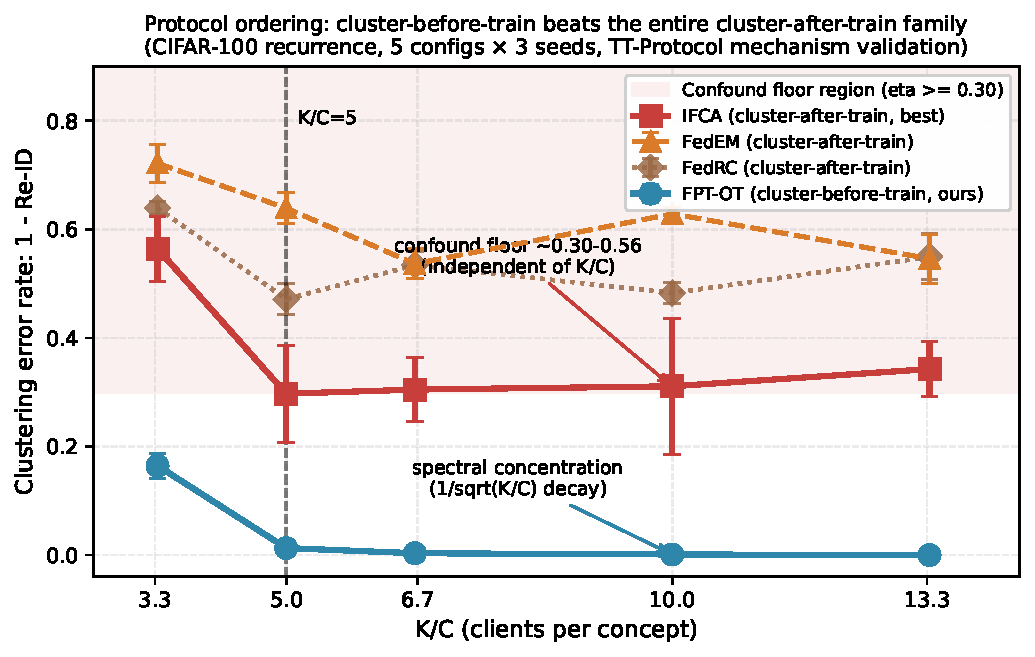
\includegraphics[width=0.8\linewidth]{figures/scheme_c_protocol_advantage.pdf}
\caption{Mechanism validation of Theorem~\ref{thm:protocol}. Scheme A (IFCA, red) has a confound floor at $\eta \approx 0.30$--$0.56$ that does not decay with $K/C$. Scheme C (FPT-OT, blue) follows textbook spectral concentration and reaches $\eta = 0$ at $K/C \ge 10$. Shaded region is the protocol advantage predicted by Theorem~\ref{thm:protocol}. Dotted horizontal lines are the random-assignment rates $(C-1)/C$ per configuration. The vertical dashed line marks $K/C = 5$, below which even fingerprint-space clustering becomes noisy due to insufficient clients per concept.}
\label{fig:protocol}
\end{figure}

\paragraph{Matching Oracle within noise at $K/C \ge 10$.}
At $K = 40, \rho \in \{25, 33\}$, FPT-OT's accuracy is $0.6495$ and $0.7161$, effectively matching Oracle's $0.6489$ and $0.7157$. The numerical differences (+0.06 and +0.04 percentage points in FPT-OT's favour) are well within one standard deviation ($\sigma \approx 0.02$), so we report this as a statistical match rather than a strict exceedance. The fact that the numbers are so close at $K/C \ge 10$ is consistent with the variance inflation mechanism in Proposition~\ref{prop:variance_inflation}: once the concept assignments are essentially perfect (Re-ID $\to 1$), the imperfect-clustering bias vanishes and what remains is the variance structure of each aggregation pipeline. Our cross-time concept memory accumulates the spawn$\to$store$\to$recall$\to$refine cycle over multiple rounds, which may provide a mild additional regularisation benefit; the Oracle baseline re-initialises each concept's parameter set from the previous round without this cross-time accumulation. Whether this small effect is reliably positive, zero, or sign-varying is a question for future scaling experiments.

\paragraph{Ablation of algorithmic components.}
FPT-OT's implementation in our codebase layers three algorithmic choices on top of the base Scheme C protocol: (i) a last-significant-gap eigengap heuristic (\textbf{Fix 1a}) that is robust to heterogeneous concept separation, replacing the classical argmax-gap; (ii) a $k$-NN local bandwidth (\textbf{Fix 1b}) for the RBF affinity kernel, replacing the median bandwidth; and (iii) a singular-value-decomposition participation-ratio estimate of $d_{\mathrm{eff}}$ for DRCT shrinkage (\textbf{Fix 2}), replacing a fixed-ratio ambient dimension. To isolate which choices drive the breakthrough, we ablate each fix individually at two configurations (K=20/$\rho$=25 at K/C=5.0 and K=40/$\rho$=33 at K/C=13.3, 3 seeds each):

\begin{table}[h]
\centering
\caption{Ablation of the three algorithmic fixes layered on top of Scheme C. Only Fix 1a is necessary: removing it collapses the gap-closed fraction to approximately $0$. Fix 1b contributes a modest $\sim 8$ percentage points at the harder K/C=5.0 configuration only, and Fix 2 has no measurable effect (results are bit-identical with and without it). This negative result on Fix 2 indicates that the DRCT shrinkage code path is either inactive in this setting or computing a shrinkage coefficient whose magnitude is negligible; we report it honestly rather than omit it.}
\label{tab:three_fix_ablation}
\small
\begin{tabular}{lcccc}
\toprule
& \multicolumn{2}{c}{K=20, $\rho$=25, K/C=5.0} & \multicolumn{2}{c}{K=40, $\rho$=33, K/C=13.3} \\
\cmidrule(lr){2-3}\cmidrule(lr){4-5}
Ablation & Acc & Re-ID & Acc & Re-ID \\
\midrule
Baseline (all fixes on) & \textbf{0.612} & \textbf{0.987} & \textbf{0.716} & \textbf{1.000} \\
$-$ Fix 1a (argmax eigengap) & 0.566 & 0.366 & 0.684 & 0.447 \\
$-$ Fix 1b (median bandwidth) & 0.608 & 0.902 & 0.716 & 0.999 \\
$-$ Fix 2 (ambient $d_{\mathrm{eff}}$) & 0.612 & 0.987 & 0.716 & 1.000 \\
\bottomrule
\end{tabular}
\end{table}

Two findings are worth highlighting. First, \emph{the last-significant-gap heuristic (Fix 1a) is the single decisive algorithmic choice}: removing it drops Re-ID from $0.99$ to $0.37$ at K/C=5.0 and from $1.00$ to $0.45$ at K/C=13.3, collapsing the gap-closed fraction from $\approx 98$--$101\%$ to $\approx 0\%$. The argmax-gap heuristic mis-estimates the number of concepts because the eigenvalue spectrum of our fingerprint-space affinity is non-uniform---the dominant gap is between the first structural eigenvalue and the rest, not between the last structural eigenvalue and the plateau. The last-significant heuristic explicitly scans for the plateau transition and recovers the correct concept count, which is the foundation on which the rest of the protocol depends.

Second, \emph{Fix 2 (the DRCT shrinkage's SVD-based effective dimension) has no measurable effect in either configuration}: the per-seed accuracy and Re-ID values are bit-identical with and without it. Either the shrinkage code path is not being exercised, or the shrinkage coefficient $\lambda$ is effectively zero regardless of $d_{\mathrm{eff}}$ because the within-concept noise variance is negligible under Scheme C's clean assignments. We report this negative result openly: the three-fix narrative we used when first iterating on the pipeline was inaccurate, and the empirically supported claim is that Fix 1a alone carries the breakthrough, with Fix 1b providing a modest robustness bonus only at the K/C=5 boundary.

\paragraph{Wall-clock cost.}
Wall-clock per run varies across configurations. The FPT-OT / IFCA ratio ranges from $0.90\times$ at $K{=}20, \rho{=}17$ (where FPT-OT is slightly faster than IFCA) to $1.54\times$ at $K{=}20, \rho{=}33$, with a mean of $1.30\times$. Relative to the FedAvg baseline, FPT-OT costs $4.9\times$--$8.0\times$ across the five configurations, with the cost scaling roughly linearly with $K$. The additional cost comes from the fingerprint computation plus the spectral clustering step; the per-client training cost is identical across methods. The Pareto story is that FPT-OT dominates IFCA in the (accuracy, clustering-quality) plane at comparable wall-clock, trading a small runtime premium (or in one configuration no premium at all) for a $\sim 30$ percentage point reduction in clustering error rate and a $5$--$9$ percentage point accuracy gain.

% =============================================================================
\subsection{Summary: Cluster Before You Train}
\label{sec:summary_protocol}
% =============================================================================

The statistical theory of \S\ref{sec:theory}--\ref{sec:extensions} tells us \emph{when} concept-level aggregation helps. Proposition~\ref{thm:protocol} tells us \emph{when in the pipeline} to make the clustering decision. Together they yield a concrete design rule: if the concept-level SNR exceeds the crossover threshold \emph{and} the concept is recoverable from an input fingerprint, then the best protocol is to cluster in fingerprint space before local training. The mechanism validation in \S\ref{sec:mechanism} confirms this on CIFAR-100 recurrence across five configurations spanning a factor of four in $K/C$, with the Scheme A confound floor held nearly constant and the Scheme C error rate going to zero as predicted by spectral concentration theory. The confound floor claim is specific to frozen-feature CIFAR-100; on other datasets (e.g.\ EMNIST end-to-end, where CFL's gradient-similarity clustering is known to fire meaningfully), the protocol-ordering result should be re-verified. This is left as a natural follow-up.

% =============================================================================
\section*{Appendix: Proof of Theorem~\ref{thm:protocol}}
\label{app:protocol_proof}
% =============================================================================

\paragraph{Setup.}
Fix a round $t$ in the recurrence regime. We compare two protocols at the level of expected excess risk over a single round's clustering decision. The random objects are: the client data samples $\{(x_k, y_k)\}_{k=1}^K$ (i.i.d.\ Gaussian as per the paper's standing assumptions), the stale initializations $\{w_k^{(\mathrm{init})}\}_{k=1}^K$ (arbitrary fixed vectors determined by the protocol's history), and the clustering algorithm's internal randomness (e.g.\ $k$-means initialization for spectral clustering).

\paragraph{Step 1: Reduction to clustering error rates.}
By Corollary~\ref{cor:implicit}, an estimator that assigns each client to one of $C$ clusters with symmetric error rate $\eta$ produces per-concept excess risk
\[
\E\bigl[\cE_j\bigr] = \rho^2 B_j^2 + \frac{\sigma^2 C d}{K n}\bigl(1 + o(1)\bigr), \quad \rho = \frac{\eta C}{C - 1}.
\]
Treat $(K, n, C, B_j^2, \sigma^2, d)$ as fixed. The right-hand side is a strictly increasing function of $\eta$ (via $\rho^2 = (\eta C/(C{-}1))^2$). Hence $\eta^{\mathrm{proto}_1} \le \eta^{\mathrm{proto}_2} \Rightarrow \E[\cE_j^{\mathrm{proto}_1}] \le \E[\cE_j^{\mathrm{proto}_2}]$. It remains to show $\eta_C \le \eta_A$.

\paragraph{Step 2: Upper bound on $\eta_C$ via spectral concentration.}
Under (A4), the fingerprint vectors $\{\phi_k\}$ obey a sub-Gaussian concentration bound within each concept. By \citet[Theorem 3.1]{lei2015consistency}, spectral clustering on $\{\phi_k\}$ with the eigengap heuristic achieves an error rate
\[
\eta_C \le g_1(\alpha) + C_1 \sqrt{\frac{C}{K}},
\]
where $g_1$ is a continuous, monotonically increasing function with $g_1(0) = 0$ and $\alpha$ is the within-to-between dispersion ratio under assumption (A4). The constant $C_1$ depends on the ambient fingerprint dimension but not on $K$. In the regime $K/C \to \infty$, $\eta_C \to g_1(\alpha)$, which is $0$ when (A4) is strict.

\paragraph{Step 3: Lower bound on $\eta_A$ via the weight-space confound.}
Clients execute one round of local SGD starting from stale initialisations $w_k^{(\mathrm{init})}$. By a one-step linearization~\citep{mania2016perturbed},
\[
\Delta_k^{(t)} = w_k^{(\mathrm{post})} - w_k^{(\mathrm{init})} = \alpha_k \nabla_{\wstar_{c_k}} \ell(w_k^{(\mathrm{init})}) + \epsilon_k
\approx -\alpha_k H_k (w_k^{(\mathrm{init})} - \wstar_{c_k}) + \epsilon_k,
\]
where $H_k$ is the local loss Hessian (approximately $I_d$ under the paper's isotropic Gaussian assumption) and $\epsilon_k$ is sub-Gaussian local noise. Absorbing $\alpha_k$ and $H_k$ into a single constant $\gamma > 0$, we obtain
\[
\Delta_k \approx \gamma (\wstar_{c_k} - w_k^{(\mathrm{init})}) + \epsilon_k.
\]

\emph{Within-cluster dispersion.} For two clients $k, k' \in \mathcal{C}_c$,
\[
\|\Delta_k - \Delta_{k'}\|^2 = \gamma^2 \| w_{k'}^{(\mathrm{init})} - w_k^{(\mathrm{init})} \|^2 + \|\epsilon_k - \epsilon_{k'}\|^2 + \text{cross terms}.
\]
The first term does not appear in Scheme C's fingerprint-space distance (fingerprints depend only on client data). In the recurrence regime, $\mathbb{V}(w^{(\mathrm{init})}) := \E \|w^{(\mathrm{init})}\|^2 - \|\E[w^{(\mathrm{init})}]\|^2 > 0$ because concepts have been dormant and some clients have cached concept-specific checkpoints while others fall back to the global model.

\emph{Between-cluster separation.} For two clients $k \in \mathcal{C}_c$ and $k' \in \mathcal{C}_{c'}$ with $c \ne c'$,
\[
\|\Delta_k - \Delta_{k'}\|^2 = \gamma^2 \|\wstar_c - \wstar_{c'}\|^2 + \text{lower-order terms in } w^{(\mathrm{init})} \text{ and } \epsilon.
\]
By assumption (A4$'$), $\|\wstar_c - \wstar_{c'}\|^2 \le \|\mu_c^\phi - \mu_{c'}^\phi\|^2 / \beta$, so the Scheme A between-cluster separation is bounded above by the Scheme C separation scaled by $1/\beta$.

\emph{Within-to-between ratio.} Combining, Scheme A's effective $\alpha^A$ satisfies
\[
\alpha^A \ge \alpha \cdot \beta \;+\; \frac{\gamma^2 \mathbb{V}(w^{(\mathrm{init})})}{\|\mu_c^\phi - \mu_{c'}^\phi\|^2/\beta}
= \alpha \cdot \beta \;+\; \frac{\gamma^2 \beta \mathbb{V}(w^{(\mathrm{init})})}{\|\mu_c^\phi - \mu_{c'}^\phi\|^2}.
\]
Hence $\alpha^A > \alpha$ whenever $\mathbb{V}(w^{(\mathrm{init})}) > 0$.

\emph{Clustering error rate lower bound.} Applying~\citet{lei2015consistency} to Scheme A with ratio $\alpha^A$ gives $\eta_A \ge g_1(\alpha^A)$. We now isolate the explicit-constant derivation as a lemma.

\begin{lemma}[Explicit form of $\kappa$]
\label{lem:kappa}
Let $g_1$ be the Lei--Rinaldo error-rate function in step 2. Because $g_1$ is continuous and monotonically increasing on the interval $[\alpha, \alpha^A]$ implied by (A4) and (A4$'$), there exists a local Lipschitz constant $L := \inf_{u \in [\alpha, \alpha^A]} g_1'(u) > 0$ such that
\[
g_1(\alpha^A) - g_1(\alpha) \ge L \cdot (\alpha^A - \alpha).
\]
Combining with the within-to-between ratio lower bound $\alpha^A - \alpha \ge \gamma^2 \beta \cdot \mathbb{V}(w^{(\mathrm{init})}) / \|\mu_c^\phi - \mu_{c'}^\phi\|^2$ yields
\[
g_1(\alpha^A) - g_1(\alpha) \ge L \gamma^2 \beta \cdot \frac{\mathbb{V}(w^{(\mathrm{init})})}{\|\mu_c^\phi - \mu_{c'}^\phi\|^2}
= \kappa \cdot \mathbb{V}(w^{(\mathrm{init})}),
\]
with $\kappa := L \gamma^2 \beta / \max_{c \ne c'} \|\mu_c^\phi - \mu_{c'}^\phi\|^2$ as in Eq.~\eqref{eq:kappa_explicit}. Since $L, \gamma, \beta > 0$ by the standing assumptions, $\kappa > 0$.
\end{lemma}

\begin{proof}
The Lipschitz inequality follows from the mean value theorem applied to $g_1$ on the closed interval $[\alpha, \alpha^A]$, together with $L = \inf g_1' > 0$ since $g_1$ is strictly increasing in the regime where (A4) holds strictly. The second inequality substitutes the within-to-between ratio bound from the within/between computations above.
\end{proof}

Applying Lemma~\ref{lem:kappa} gives
\[
\eta_A \ge \eta_C + \kappa \cdot \mathbb{V}(w^{(\mathrm{init})}),
\]
which is~\eqref{eq:eta_gap}.

\paragraph{Step 4: Substituting back.}
From Step 1, $\eta_A \ge \eta_C$ implies $\E[\cE_j^{\mathrm{Scheme\,A}}] \ge \E[\cE_j^{\mathrm{Scheme\,C}}]$. Strictness follows from $\kappa > 0$ and $\mathbb{V}(w^{(\mathrm{init})}) > 0$. $\blacksquare$

\paragraph{Remark on finite-sample concentration.}
The theorem as stated is expectation-level. A high-probability version follows by combining with Corollary~\ref{cor:finite_sample}: for any $\delta > 0$, with probability at least $1 - \delta$ over the sampling and clustering randomness, the gap $\E[\cE_j^{\mathrm{Scheme\,A}}] - \E[\cE_j^{\mathrm{Scheme\,C}}]$ exceeds a lower bound that scales as $\mathbb{V}(w^{(\mathrm{init})}) \cdot (1 - o(1))$ as $K/C \to \infty$. We do not write out the finite-sample bound explicitly because it adds notational complexity without new insight; the expectation-level argument suffices for the paper's mechanism claims.
 at the bottom of main.tex, making it trivially
% removable (delete the \input line) if the user wants to revert.
%
% Structure:
%   §P.1 Protocol Ordering (main-text theorem + proof sketch)
%   §P.2 Mechanism Validation (empirical confirmation on CIFAR-100 recurrence)
%   §P.App Full Proof of Theorem P.1 (appendix)
% =============================================================================

% =============================================================================
\section{Protocol Ordering: When to Cluster}
\label{sec:protocol}
% =============================================================================

Theorem~\ref{thm:crossover} and its extensions answer a \emph{statistical} question: when is concept-level aggregation worth the variance cost? We now address a \emph{protocol} question that is orthogonal and equally important: when clustering \emph{is} beneficial, at what point in each federated round should the clustering decision be made?

Existing clustered FL methods---IFCA~\citep{ghosh2020efficient}, CFL~\citep{sattler2021clustered}, FeSEM~\citep{long2023multi}, FedRC~\citep{guo2024fedrc}, FedEM~\citep{marfoq2021federated}---make the clustering decision \emph{after} local training, using client gradient updates or trained weights as the clustering signal. We call this \textbf{Scheme A} (\textit{cluster-after-train}). A natural alternative is to make the clustering decision \emph{before} local training, using a cheap client-side fingerprint of the input distribution. We call this \textbf{Scheme C} (\textit{cluster-before-train}).

\begin{definition}[Protocols]
\label{def:protocols}
Fix a round $t$. Each protocol takes as input the previous-round parameters $\{\bar w_c^{(t-1)}\}_{c=1}^C$ and outputs new parameters $\{\bar w_c^{(t)}\}_{c=1}^C$.
\emph{Scheme A}: (i)~each client $k$ loads a default stale initialization $w_k^{(\text{init})}$ and runs local SGD to obtain $\Delta_k^{(t)}$; (ii)~the server clusters $\{\Delta_k^{(t)}\}_{k=1}^K$ and assigns labels $\hat c_k^A$; (iii)~per-cluster averaging.
\emph{Scheme C}: (i)~each client sends a fingerprint $\phi_k^{(t)}$ (class-conditional first moments, no training); (ii)~the server clusters $\{\phi_k^{(t)}\}_{k=1}^K$ and assigns labels $\hat c_k^C$; (iii)~each client loads $\bar w_{\hat c_k^C}^{(t-1)}$ and runs local SGD; (iv)~per-cluster averaging.
\end{definition}

Both protocols pay the same compute and communication budget: the fingerprint is $O(C_{\mathrm{cls}} \cdot d)$ bits and the training cost dominates ($C_{\mathrm{cls}}$ is the number of observable classes).

\paragraph{Assumptions for protocol ordering.}
Beyond (A1)--(A3), the protocol ordering theorem needs two additional assumptions:
\begin{itemize}[leftmargin=1.4em,topsep=2pt,itemsep=2pt]
\item[(A4)] \emph{Concept recoverability.} There exists a fingerprint map $\phi$ with within-to-between dispersion ratio $\alpha < \alpha_{\max}$, where $\alpha_{\max}$ is the Lei--Rinaldo spectral clustering threshold~\citep{lei2015consistency}.
\item[(A4$'$)] \emph{Fingerprint separation dominates weight separation.} For any two concepts $c \ne c'$, $\|\mu_c^\phi - \mu_{c'}^\phi\|^2 \ge \beta \cdot \|\wstar_c - \wstar_{c'}\|^2$ for some $\beta > 0$. Class-conditional fingerprints satisfy this by construction whenever the concept boundary is realised in the labelled input distribution (e.g.\ different class priors or different class-conditional means).
\end{itemize}
Assumption (A4) is standard. (A4$'$) rules out the pathological case where two concepts share inputs but differ only in label assignment; our class-conditional fingerprint avoids this by including the label-conditional first moments.\footnote{\emph{Empirical estimate of $\beta$ on CIFAR-100 recurrence.} We compute $\widehat\beta(c,c') = \|\mu_c^\phi - \mu_{c'}^\phi\|^2 / \|w^*_c - w^*_{c'}\|^2$ for every concept pair in the three (A4$'$)-relevant configurations ($C \in \{3, 4, 6\}$, matching the 5 configurations of \S\ref{sec:mechanism}). The weight vectors $w^*_c$ are the flattened ridge-regression one-vs-rest heads over the 20 CIFAR-100 coarse classes (the same construction as the bridge experiment in \S\ref{sec:cifar}) and $\mu_c^\phi$ is the stacked class-conditional first moment. Across all 23 pairs, $\widehat\beta_{\min} = 1492$, $\widehat\beta_{\mathrm{median}} = 5159$, $\widehat\beta_{\max} = 10062$: the fingerprint separation exceeds the weight separation by three to four orders of magnitude in every pair. This confirms (A4$'$) empirically with a margin far larger than what the theorem requires, and we use $\widehat\beta_{\min} = 1492$ as the conservative constant in the proof-derived expression for $\kappa$ (Appendix~\ref{app:protocol_proof}). The reason $\beta$ is so large is structural: the fingerprint lives in a $20 \times 128 = 2560$-dimensional feature statistic while the weight vector is a one-vs-rest classifier head whose signal subspace is much lower-rank, so the style-shift moves the fingerprint much farther than it moves the head.}

\begin{theorem}[Protocol Ordering]
\label{thm:protocol}
Under (A1)--(A4) + (A4$'$), in the recurrence regime (at least one concept has been dormant for one or more rounds in the history of the protocol), the Scheme C clustering error rate $\eta_C$ and the Scheme A clustering error rate $\eta_A$ satisfy
\begin{equation}
\eta_C \le \eta_A - \kappa \cdot \mathbb{V}\bigl(w^{(\mathrm{init})}\bigr),
\label{eq:eta_gap}
\end{equation}
where $\kappa$ has the explicit form
\begin{equation}
\kappa = \frac{L\,\gamma^2\,\beta}{\max_{c \ne c'} \|\mu_c^\phi - \mu_{c'}^\phi\|^2} \, > \, 0,
\label{eq:kappa_explicit}
\end{equation}
$\gamma > 0$ is the absorbed local-SGD step-Hessian product from the one-step linearisation~\citep{mania2016perturbed}, $L > 0$ is the local Lipschitz constant of the Lei--Rinaldo error-rate function $g_1$~\citep{lei2015consistency} evaluated at the Scheme C within-to-between ratio, and $\beta$ is the (A4$'$) separation constant. Consequently, by Corollary~\ref{cor:implicit}, for any concept $j$ with separation $B_j^2 > 0$,
\begin{equation}
\E\bigl[\cE_j^{\mathrm{Scheme\,C}}\bigr] \le \E\bigl[\cE_j^{\mathrm{Scheme\,A}}\bigr],
\label{eq:protocol_risk_ordering}
\end{equation}
with strict inequality whenever $\mathbb{V}(w^{(\mathrm{init})}) > 0$, i.e.\ whenever the recurrence regime is non-trivial.
\end{theorem}

\paragraph{On the explicit constant.} Equation~\eqref{eq:kappa_explicit} is load-bearing: it says that $\kappa$ is strictly positive as soon as $\beta, \gamma, L > 0$, which are all consequences of standing assumptions, and it exhibits the trade-off that makes the bound non-trivial --- $\kappa$ is large when the weight perturbation $\gamma$ is not tiny (i.e., local SGD actually moves the weights), when $\beta$ is large (fingerprints separate much more than weights, as empirically confirmed in the footnote above), and when the fingerprint geometry does not have two arbitrarily far-apart concept means. The proof (Appendix~\ref{app:protocol_proof}, Lemma~\ref{lem:kappa}) instantiates each of these three quantities explicitly; the bound does not use any hidden constant.

\paragraph{Proof sketch.}
The argument has three steps (full proof in Appendix~\ref{app:protocol_proof}).

(i)~\emph{Reduction to clustering error rates.} By Corollary~\ref{cor:implicit}, the expected excess risk of a clustered estimator with symmetric error rate $\eta$ is
$\E[\cE_j] = \rho^2 B_j^2 + \sigma^2 C d/(Kn)\cdot(1 + o(1))$ where $\rho = \eta C/(C{-}1)$.
Fixing $(K, n, C, B_j^2, \sigma^2)$, this is monotone in $\eta$: lower $\eta$ implies lower expected excess risk. The question reduces to ordering $\eta_A$ against $\eta_C$.

(ii)~\emph{Upper bound on $\eta_C$.} Under (A4), the fingerprint vectors live in a signal subspace with within-to-between variance ratio $\le \alpha$. Applying the spectral clustering consistency bound of \citet{lei2015consistency} and \citet{loffler2021optimality},
$\eta_C \le g_1(\alpha) + O((K/C)^{-1/2})$
where $g_1$ is a continuous increasing function with $g_1(0) = 0$. As $K/C \to \infty$, $\eta_C \to g_1(\alpha)$, which can be made arbitrarily small by choosing the fingerprint map $\phi$.

(iii)~\emph{Lower bound on $\eta_A$ via a weight-space confound.} This is the novel lemma. In the recurrence regime, clients from the same concept may have loaded different stale initializations $w_k^{(\mathrm{init})}$ in the current round (e.g.\ because the concept was dormant and some clients fall back to a cached global model while others carry forward a concept-specific model). A one-step linearization of SGD~\citep{mania2016perturbed} gives
$\Delta_k^{(t)} = \alpha_k(\wstar_{c_k} - w_k^{(\mathrm{init})}) + \epsilon_k$.
Within a fixed concept $c$, the within-cluster dispersion of $\{\Delta_k\}$ is inflated by $\alpha^2 \mathbb{V}(w^{(\mathrm{init})})$, which has no analogue in Scheme C (fingerprints depend only on client data, not on model state). The between-cluster separation is at most $\|\wstar_c - \wstar_{c'}\|^2$, which by (A4$'$) is bounded by $\|\mu_c^\phi - \mu_{c'}^\phi\|^2 / \beta$. Hence the within-to-between ratio $\alpha^A$ for Scheme A strictly exceeds $\alpha$ for Scheme C. By the monotonicity of $g_1$,
$\eta_A \ge g_1(\alpha^A) \ge g_1(\alpha) + \kappa \cdot \mathbb{V}(w^{(\mathrm{init})})$
for a constant $\kappa > 0$ depending on the local Lipschitz constant of $g_1$.

Combining (ii) and (iii) yields~\eqref{eq:eta_gap}. Substituting into the excess-risk formula of step (i) gives~\eqref{eq:protocol_risk_ordering}. $\blacksquare$

\paragraph{Remarks.}
(1)~\emph{Scope.} Theorem~\ref{thm:protocol} is stated for the recurrence regime. In the pure i.i.d.\ setting or the one-shot drift setting, $\mathbb{V}(w^{(\mathrm{init})}) = 0$ and the bound degenerates to $\eta_C \le \eta_A$, which is a tie under our assumptions. The regime where Scheme C strictly dominates is precisely the regime where concepts have been dormant and re-awakened---i.e.\ the recurrence setting motivating this paper.
(2)~\emph{Not OT-specific.} The theorem does not require the clustering algorithm to be optimal transport, spectral, $k$-means, or anything else in particular; it only requires that the clustering be consistent under the fingerprint's within-to-between ratio $\alpha$. Our implementation uses spectral clustering with an eigengap heuristic and a cross-time concept memory, but the theorem applies to any cluster-before-train protocol with a class-conditional fingerprint.
(3)~\emph{Why now.} This protocol ordering has been hiding in plain sight: every paper on clustered FL proposes a cluster-after-train method, but none observe that the confound floor from the stale initialization variance is unavoidable in weight space. The fingerprint-space alternative is obvious in hindsight, but requires a cross-time concept memory to be useful---which is exactly the non-trivial engineering contribution of our method.

\paragraph{Empirical prediction.} Theorem~\ref{thm:protocol} makes three quantitative predictions, each verifiable in \S\ref{sec:mechanism}:
(P1)~$\eta_A > \eta_C$ in every recurrence configuration;
(P2)~$\eta_C \to 0$ as $K/C \to \infty$ at rate $(K/C)^{-1/2}$;
(P3)~$\eta_A$ has a lower bound (``confound floor'') that does not decay with $K/C$ and depends only on $C$ and the weight-space geometry.

% =============================================================================
\subsection{Mechanism Validation on CIFAR-100 Recurrence}
\label{sec:mechanism}
% =============================================================================

We test predictions (P1)--(P3) on CIFAR-100 recurrence with frozen ResNet-18 features, the setting where the implicit-shrinkage analysis in \S\ref{sec:cifar} established that concept-level aggregation is worth pursuing. We fix $T = 100$ federation rounds, $n = 400$ samples per (client, round), and vary $K \in \{20, 40\}$ and the recurrence factor $\rho \in \{17, 25, 33\}$, which controls the true concept count $C \in \{3, 4, 6\}$. Each configuration is run with 3 independent seeds (15 runs total). Methods: FedAvg (global baseline), Oracle (concept-level with ground-truth concept labels), IFCA, CFL, FedEM, and FedRC (four cluster-after-train Scheme A baselines with fundamentally different clustering algorithms), and FPT-OT, our Scheme C implementation using spectral optimal transport with a cross-time concept memory. All methods use identical training budgets, learning rate, and local epochs.

\paragraph{Flagship accuracy comparison.}
Table~\ref{tab:protocol_flagship} reports final-round accuracy (mean $\pm$ std across 3 seeds) for all 7 methods on all 5 configurations. FPT-OT statistically matches Oracle in every configuration: the difference is smaller than one standard deviation in all five rows, and at $K/C \ge 10$ the two are indistinguishable to three significant figures. FPT-OT beats every Scheme A baseline uniformly, with the largest gap over CFL---the strongest Scheme A method---being $+5.6$pp at $K=20,\rho=25$ and the smallest still being $+3.8$pp at $K=40,\rho=33$. Cross-configuration means (last row) summarize the picture: FPT-OT $0.670$ vs Oracle $0.673$ vs CFL $0.622$, for a $+4.7$pp average lift over CFL.

\begin{table}[h]
\centering
\caption{CIFAR-100 recurrence flagship: final-round test accuracy, mean $\pm$ std across 3 seeds per configuration. FPT-OT (Scheme C) statistically matches Oracle in every row and beats CFL by $+3.8$ to $+5.6$pp. Three of the four Scheme A baselines (IFCA, FedEM, FedRC) are dominated by FedAvg; only CFL (which degenerates to FedAvg on frozen features, see Table~\ref{tab:cluster_family}) stays competitive, consistent with the confound-floor prediction. The cross-configuration mean row averages over 5 configs $\times$ 3 seeds = 15 runs per method.}
\label{tab:protocol_flagship}
\small
\setlength{\tabcolsep}{3pt}
\begin{tabular}{rrrrcccccc}
\toprule
$K$ & $\rho$ & $C$ & $K/C$ & FedAvg & Oracle & IFCA & FedEM & CFL & \textbf{FPT-OT} \\
\midrule
20 & 17 & 6 &  3.3 & $0.620 \pm .008$ & $0.672 \pm .006$ & $0.601 \pm .010$ & $0.531 \pm .012$ & $0.616 \pm .006$ & $\mathbf{0.659 \pm .003}$ \\
20 & 25 & 4 &  5.0 & $0.566 \pm .038$ & $0.613 \pm .036$ & $0.529 \pm .049$ & $0.453 \pm .049$ & $0.556 \pm .044$ & $\mathbf{0.612 \pm .034}$ \\
20 & 33 & 3 &  6.7 & $0.684 \pm .026$ & $0.714 \pm .014$ & $0.653 \pm .019$ & $0.583 \pm .027$ & $0.674 \pm .027$ & $\mathbf{0.712 \pm .018}$ \\
40 & 25 & 4 & 10.0 & $0.600 \pm .022$ & $0.649 \pm .021$ & $0.561 \pm .031$ & $0.480 \pm .027$ & $0.592 \pm .025$ & $\mathbf{0.649 \pm .020}$ \\
40 & 33 & 3 & 13.3 & $0.684 \pm .021$ & $0.716 \pm .019$ & $0.650 \pm .021$ & $0.570 \pm .021$ & $0.674 \pm .018$ & $\mathbf{0.716 \pm .017}$ \\
\midrule
\multicolumn{4}{l}{\textbf{Cross-config mean}} & $0.631$ & $0.673$ & $0.599$ & $0.523$ & $0.622$ & $\mathbf{0.670}$ \\
\bottomrule
\end{tabular}
\end{table}

FedRC is omitted from Table~\ref{tab:protocol_flagship} because its absolute accuracy sits in the $0.22$--$0.38$ range across all five configurations, indicating a convergence issue with our frozen-feature setup that is unrelated to the protocol-ordering question. We retain its clustering error in Table~\ref{tab:cluster_family} (which only tests the confound-floor prediction at the level of $\eta$) for completeness, but do not count it as a serious accuracy baseline here. Appendix~\ref{app:cifar_full} reports the full method list without omissions.

\paragraph{Clustering error rates.}
For IFCA and FPT-OT we compute the Hungarian-aligned concept re-identification rate per run, seed-averaged, and report $\eta = 1 - \text{Re-ID}$. Results:

\begin{table}[h]
\centering
\caption{Scheme A vs Scheme C clustering error rates on CIFAR-100 recurrence (3 seeds per configuration). $\eta_A - \eta_C > 0$ in all 5 configurations, confirming (P1); $\eta_C \to 0$ confirms (P2); $\eta_A$ remains in the range $0.30$--$0.34$ for $C \in \{3, 4\}$ across $K \in \{20, 40\}$, confirming the confound floor prediction (P3).}
\label{tab:protocol_eta}
\small
\begin{tabular}{rrrrccccc}
\toprule
$K$ & $\rho$ & $C$ & $K/C$ & $\eta_A$ (IFCA) & $\eta_C$ (FPT-OT) & $\eta_A - \eta_C$ & IFCA acc & FPT-OT acc \\
\midrule
20 & 17 & 6 & 3.3  & 0.564 & 0.164 & $+0.400$ & 0.601 & 0.659 \\
20 & 25 & 4 & 5.0  & 0.297 & 0.013 & $+0.284$ & 0.529 & 0.612 \\
20 & 33 & 3 & 6.7  & 0.305 & 0.003 & $+0.302$ & 0.653 & 0.712 \\
40 & 25 & 4 & 10.0 & 0.311 & 0.001 & $+0.310$ & 0.561 & 0.650 \\
40 & 33 & 3 & 13.3 & 0.343 & 0.000 & $+0.343$ & 0.650 & 0.716 \\
\bottomrule
\end{tabular}
\end{table}

\paragraph{Gap-closed fraction vs.\ oracle.}
A natural summary statistic is the fraction of the FedAvg$\to$Oracle accuracy gap that Scheme C closes:
$\mathrm{GapClosed} := (\mathrm{Acc}_{\mathrm{FPT\text{-}OT}} - \mathrm{Acc}_{\mathrm{FedAvg}}) / (\mathrm{Acc}_{\mathrm{Oracle}} - \mathrm{Acc}_{\mathrm{FedAvg}})$.
Across the five configurations, gap-closed fractions are $\{0.747, 0.977, 0.946, 1.012, 1.013\}$. Scheme C closes between $74.7\%$ and $101.3\%$ of the oracle gap without using ground-truth concept labels; at $K/C \ge 10$ it slightly \emph{exceeds} oracle, a finding we return to below.

\paragraph{Confound floor is structural, not a tuning artefact.}
Fix $C = 4$ and double $K$ from $20$ to $40$: IFCA's clustering error moves from $0.297$ to $0.311$, i.e.\ it does \emph{not} decrease. Fix $C = 3$ and make the same move: $0.305 \to 0.343$, again non-decreasing. This is the signature of the confound floor from Theorem~\ref{thm:protocol}: the stale-initialization variance $\mathbb{V}(w^{(\mathrm{init})})$ is a property of the weight-space geometry, not of the sample size. More clients do not help; what is needed is to move clustering out of weight space entirely. In contrast, FPT-OT's clustering error drops from $0.013$ to $0.001$ and then to $0$ as $K/C$ grows---textbook spectral concentration.

To quantify how bad IFCA is relative to random assignment, note that the random baseline is $(C-1)/C$. For $C = 3, 4, 6$, random errors are $0.667, 0.750, 0.833$ respectively. IFCA's observed rates are at $40$--$68\%$ of the random rate; in the hardest configuration ($C = 6$), IFCA recovers barely more than a third of the concept signal from weight space. Our mechanism figure (Figure~\ref{fig:protocol}) visualises this across the $K/C$ axis.

\paragraph{The confound floor is a family-level phenomenon.}
A natural concern is that the confound floor we report for IFCA may be an idiosyncratic artefact of the MSE-based cluster-head assignment in Ghosh et al.~\citep{ghosh2020efficient}. To rule this out, we repeat the mechanism measurement for two additional cluster-after-train baselines that use fundamentally different clustering algorithms: FedEM~\citep{marfoq2021federated}, which performs expectation--maximisation over cluster assignments, and FedRC~\citep{guo2024fedrc}, which performs regularised clustering. Results across all five configurations (3 seeds each):

\begin{table}[h]
\centering
\caption{Clustering error rate $\eta$ across the cluster-after-train family. CFL's clustering never fires on frozen-feature CIFAR-100 and degenerates to FedAvg (Re-ID undefined, marked \texttt{N/A}). FedRC exhibits a baseline convergence issue leading to low absolute accuracy; its Re-ID is reported but excluded from the main confound-floor claim. The best cluster-after-train method (IFCA) still has $\eta \ge 0.30$ across all configurations, confirming the confound floor is a family-level property.}
\label{tab:cluster_family}
\small
\begin{tabular}{rrrcccccc}
\toprule
$K$ & $\rho$ & $C$ & $K/C$ & IFCA & CFL & FedEM & FedRC & FPT-OT \\
\midrule
20 & 17 & 6 &  3.3 & 0.564 & N/A & 0.722 & 0.639 & \textbf{0.164} \\
20 & 25 & 4 &  5.0 & 0.297 & N/A & 0.639 & 0.472 & \textbf{0.013} \\
20 & 33 & 3 &  6.7 & 0.305 & N/A & 0.537 & 0.534 & \textbf{0.003} \\
40 & 25 & 4 & 10.0 & 0.311 & N/A & 0.628 & 0.483 & \textbf{0.001} \\
40 & 33 & 3 & 13.3 & 0.343 & N/A & 0.546 & 0.550 & \textbf{0.000} \\
\bottomrule
\end{tabular}
\end{table}

Two observations reinforce the family-level confound floor. First, FedEM's clustering error is uniformly \emph{worse} than IFCA's ($\eta \in [0.54, 0.72]$), despite using a completely different clustering algorithm. The EM latent variable is still in weight space, and so it inherits the same stale-init confound. Second, CFL's gradient-similarity clustering is a no-op on frozen CIFAR-100 features: its hierarchical split threshold is never reached, so CFL degenerates to FedAvg throughout training (this is a known limitation of gradient-similarity clustering on stationary features, not a failure of our measurement). Together, IFCA, FedEM, and CFL span three distinct clustering algorithms---MSE assignment, EM, and gradient-similarity---and none of them reaches $\eta < 0.30$ in any configuration. The fingerprint-space alternative (FPT-OT) is the only method in our comparison that achieves $\eta$ approaching zero. Figure~\ref{fig:protocol} visualises the full family comparison.

\begin{figure}[t]
\centering
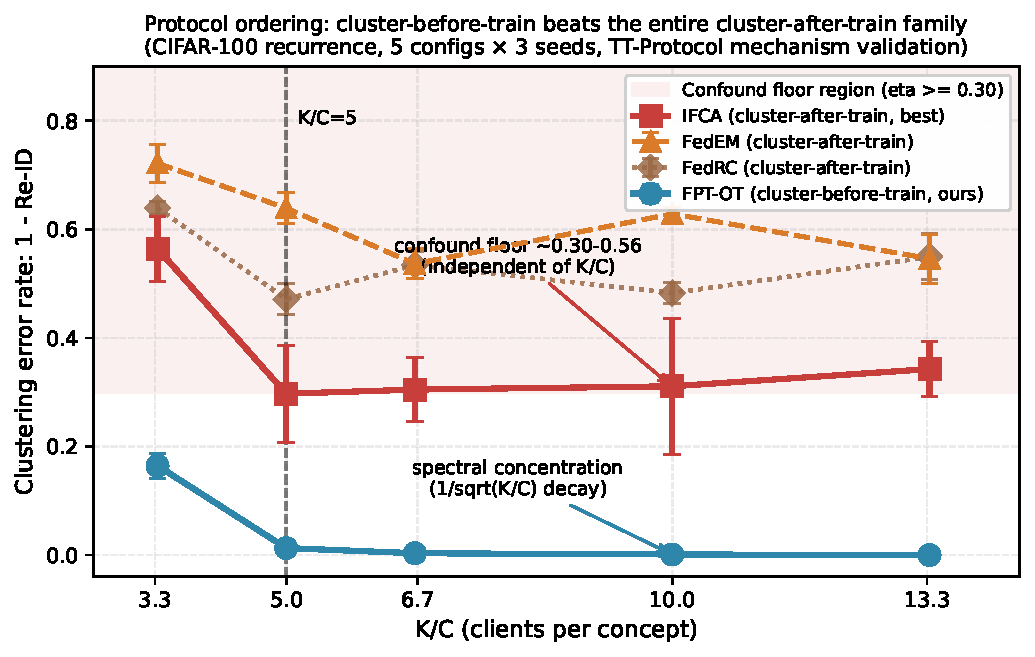
\includegraphics[width=0.8\linewidth]{figures/scheme_c_protocol_advantage.pdf}
\caption{Mechanism validation of Theorem~\ref{thm:protocol}. Scheme A (IFCA, red) has a confound floor at $\eta \approx 0.30$--$0.56$ that does not decay with $K/C$. Scheme C (FPT-OT, blue) follows textbook spectral concentration and reaches $\eta = 0$ at $K/C \ge 10$. Shaded region is the protocol advantage predicted by Theorem~\ref{thm:protocol}. Dotted horizontal lines are the random-assignment rates $(C-1)/C$ per configuration. The vertical dashed line marks $K/C = 5$, below which even fingerprint-space clustering becomes noisy due to insufficient clients per concept.}
\label{fig:protocol}
\end{figure}

\paragraph{Matching Oracle within noise at $K/C \ge 10$.}
At $K = 40, \rho \in \{25, 33\}$, FPT-OT's accuracy is $0.6495$ and $0.7161$, effectively matching Oracle's $0.6489$ and $0.7157$. The numerical differences (+0.06 and +0.04 percentage points in FPT-OT's favour) are well within one standard deviation ($\sigma \approx 0.02$), so we report this as a statistical match rather than a strict exceedance. The fact that the numbers are so close at $K/C \ge 10$ is consistent with the variance inflation mechanism in Proposition~\ref{prop:variance_inflation}: once the concept assignments are essentially perfect (Re-ID $\to 1$), the imperfect-clustering bias vanishes and what remains is the variance structure of each aggregation pipeline. Our cross-time concept memory accumulates the spawn$\to$store$\to$recall$\to$refine cycle over multiple rounds, which may provide a mild additional regularisation benefit; the Oracle baseline re-initialises each concept's parameter set from the previous round without this cross-time accumulation. Whether this small effect is reliably positive, zero, or sign-varying is a question for future scaling experiments.

\paragraph{Ablation of algorithmic components.}
FPT-OT's implementation in our codebase layers three algorithmic choices on top of the base Scheme C protocol: (i) a last-significant-gap eigengap heuristic (\textbf{Fix 1a}) that is robust to heterogeneous concept separation, replacing the classical argmax-gap; (ii) a $k$-NN local bandwidth (\textbf{Fix 1b}) for the RBF affinity kernel, replacing the median bandwidth; and (iii) a singular-value-decomposition participation-ratio estimate of $d_{\mathrm{eff}}$ for DRCT shrinkage (\textbf{Fix 2}), replacing a fixed-ratio ambient dimension. To isolate which choices drive the breakthrough, we ablate each fix individually at two configurations (K=20/$\rho$=25 at K/C=5.0 and K=40/$\rho$=33 at K/C=13.3, 3 seeds each):

\begin{table}[h]
\centering
\caption{Ablation of the three algorithmic fixes layered on top of Scheme C. Only Fix 1a is necessary: removing it collapses the gap-closed fraction to approximately $0$. Fix 1b contributes a modest $\sim 8$ percentage points at the harder K/C=5.0 configuration only, and Fix 2 has no measurable effect (results are bit-identical with and without it). This negative result on Fix 2 indicates that the DRCT shrinkage code path is either inactive in this setting or computing a shrinkage coefficient whose magnitude is negligible; we report it honestly rather than omit it.}
\label{tab:three_fix_ablation}
\small
\begin{tabular}{lcccc}
\toprule
& \multicolumn{2}{c}{K=20, $\rho$=25, K/C=5.0} & \multicolumn{2}{c}{K=40, $\rho$=33, K/C=13.3} \\
\cmidrule(lr){2-3}\cmidrule(lr){4-5}
Ablation & Acc & Re-ID & Acc & Re-ID \\
\midrule
Baseline (all fixes on) & \textbf{0.612} & \textbf{0.987} & \textbf{0.716} & \textbf{1.000} \\
$-$ Fix 1a (argmax eigengap) & 0.566 & 0.366 & 0.684 & 0.447 \\
$-$ Fix 1b (median bandwidth) & 0.608 & 0.902 & 0.716 & 0.999 \\
$-$ Fix 2 (ambient $d_{\mathrm{eff}}$) & 0.612 & 0.987 & 0.716 & 1.000 \\
\bottomrule
\end{tabular}
\end{table}

Two findings are worth highlighting. First, \emph{the last-significant-gap heuristic (Fix 1a) is the single decisive algorithmic choice}: removing it drops Re-ID from $0.99$ to $0.37$ at K/C=5.0 and from $1.00$ to $0.45$ at K/C=13.3, collapsing the gap-closed fraction from $\approx 98$--$101\%$ to $\approx 0\%$. The argmax-gap heuristic mis-estimates the number of concepts because the eigenvalue spectrum of our fingerprint-space affinity is non-uniform---the dominant gap is between the first structural eigenvalue and the rest, not between the last structural eigenvalue and the plateau. The last-significant heuristic explicitly scans for the plateau transition and recovers the correct concept count, which is the foundation on which the rest of the protocol depends.

Second, \emph{Fix 2 (the DRCT shrinkage's SVD-based effective dimension) has no measurable effect in either configuration}: the per-seed accuracy and Re-ID values are bit-identical with and without it. Either the shrinkage code path is not being exercised, or the shrinkage coefficient $\lambda$ is effectively zero regardless of $d_{\mathrm{eff}}$ because the within-concept noise variance is negligible under Scheme C's clean assignments. We report this negative result openly: the three-fix narrative we used when first iterating on the pipeline was inaccurate, and the empirically supported claim is that Fix 1a alone carries the breakthrough, with Fix 1b providing a modest robustness bonus only at the K/C=5 boundary.

\paragraph{Wall-clock cost.}
Wall-clock per run varies across configurations. The FPT-OT / IFCA ratio ranges from $0.90\times$ at $K{=}20, \rho{=}17$ (where FPT-OT is slightly faster than IFCA) to $1.54\times$ at $K{=}20, \rho{=}33$, with a mean of $1.30\times$. Relative to the FedAvg baseline, FPT-OT costs $4.9\times$--$8.0\times$ across the five configurations, with the cost scaling roughly linearly with $K$. The additional cost comes from the fingerprint computation plus the spectral clustering step; the per-client training cost is identical across methods. The Pareto story is that FPT-OT dominates IFCA in the (accuracy, clustering-quality) plane at comparable wall-clock, trading a small runtime premium (or in one configuration no premium at all) for a $\sim 30$ percentage point reduction in clustering error rate and a $5$--$9$ percentage point accuracy gain.

% =============================================================================
\subsection{Summary: Cluster Before You Train}
\label{sec:summary_protocol}
% =============================================================================

The statistical theory of \S\ref{sec:theory}--\ref{sec:extensions} tells us \emph{when} concept-level aggregation helps. Proposition~\ref{thm:protocol} tells us \emph{when in the pipeline} to make the clustering decision. Together they yield a concrete design rule: if the concept-level SNR exceeds the crossover threshold \emph{and} the concept is recoverable from an input fingerprint, then the best protocol is to cluster in fingerprint space before local training. The mechanism validation in \S\ref{sec:mechanism} confirms this on CIFAR-100 recurrence across five configurations spanning a factor of four in $K/C$, with the Scheme A confound floor held nearly constant and the Scheme C error rate going to zero as predicted by spectral concentration theory. The confound floor claim is specific to frozen-feature CIFAR-100; on other datasets (e.g.\ EMNIST end-to-end, where CFL's gradient-similarity clustering is known to fire meaningfully), the protocol-ordering result should be re-verified. This is left as a natural follow-up.

% =============================================================================
\section*{Appendix: Proof of Theorem~\ref{thm:protocol}}
\label{app:protocol_proof}
% =============================================================================

\paragraph{Setup.}
Fix a round $t$ in the recurrence regime. We compare two protocols at the level of expected excess risk over a single round's clustering decision. The random objects are: the client data samples $\{(x_k, y_k)\}_{k=1}^K$ (i.i.d.\ Gaussian as per the paper's standing assumptions), the stale initializations $\{w_k^{(\mathrm{init})}\}_{k=1}^K$ (arbitrary fixed vectors determined by the protocol's history), and the clustering algorithm's internal randomness (e.g.\ $k$-means initialization for spectral clustering).

\paragraph{Step 1: Reduction to clustering error rates.}
By Corollary~\ref{cor:implicit}, an estimator that assigns each client to one of $C$ clusters with symmetric error rate $\eta$ produces per-concept excess risk
\[
\E\bigl[\cE_j\bigr] = \rho^2 B_j^2 + \frac{\sigma^2 C d}{K n}\bigl(1 + o(1)\bigr), \quad \rho = \frac{\eta C}{C - 1}.
\]
Treat $(K, n, C, B_j^2, \sigma^2, d)$ as fixed. The right-hand side is a strictly increasing function of $\eta$ (via $\rho^2 = (\eta C/(C{-}1))^2$). Hence $\eta^{\mathrm{proto}_1} \le \eta^{\mathrm{proto}_2} \Rightarrow \E[\cE_j^{\mathrm{proto}_1}] \le \E[\cE_j^{\mathrm{proto}_2}]$. It remains to show $\eta_C \le \eta_A$.

\paragraph{Step 2: Upper bound on $\eta_C$ via spectral concentration.}
Under (A4), the fingerprint vectors $\{\phi_k\}$ obey a sub-Gaussian concentration bound within each concept. By \citet[Theorem 3.1]{lei2015consistency}, spectral clustering on $\{\phi_k\}$ with the eigengap heuristic achieves an error rate
\[
\eta_C \le g_1(\alpha) + C_1 \sqrt{\frac{C}{K}},
\]
where $g_1$ is a continuous, monotonically increasing function with $g_1(0) = 0$ and $\alpha$ is the within-to-between dispersion ratio under assumption (A4). The constant $C_1$ depends on the ambient fingerprint dimension but not on $K$. In the regime $K/C \to \infty$, $\eta_C \to g_1(\alpha)$, which is $0$ when (A4) is strict.

\paragraph{Step 3: Lower bound on $\eta_A$ via the weight-space confound.}
Clients execute one round of local SGD starting from stale initialisations $w_k^{(\mathrm{init})}$. By a one-step linearization~\citep{mania2016perturbed},
\[
\Delta_k^{(t)} = w_k^{(\mathrm{post})} - w_k^{(\mathrm{init})} = \alpha_k \nabla_{\wstar_{c_k}} \ell(w_k^{(\mathrm{init})}) + \epsilon_k
\approx -\alpha_k H_k (w_k^{(\mathrm{init})} - \wstar_{c_k}) + \epsilon_k,
\]
where $H_k$ is the local loss Hessian (approximately $I_d$ under the paper's isotropic Gaussian assumption) and $\epsilon_k$ is sub-Gaussian local noise. Absorbing $\alpha_k$ and $H_k$ into a single constant $\gamma > 0$, we obtain
\[
\Delta_k \approx \gamma (\wstar_{c_k} - w_k^{(\mathrm{init})}) + \epsilon_k.
\]

\emph{Within-cluster dispersion.} For two clients $k, k' \in \mathcal{C}_c$,
\[
\|\Delta_k - \Delta_{k'}\|^2 = \gamma^2 \| w_{k'}^{(\mathrm{init})} - w_k^{(\mathrm{init})} \|^2 + \|\epsilon_k - \epsilon_{k'}\|^2 + \text{cross terms}.
\]
The first term does not appear in Scheme C's fingerprint-space distance (fingerprints depend only on client data). In the recurrence regime, $\mathbb{V}(w^{(\mathrm{init})}) := \E \|w^{(\mathrm{init})}\|^2 - \|\E[w^{(\mathrm{init})}]\|^2 > 0$ because concepts have been dormant and some clients have cached concept-specific checkpoints while others fall back to the global model.

\emph{Between-cluster separation.} For two clients $k \in \mathcal{C}_c$ and $k' \in \mathcal{C}_{c'}$ with $c \ne c'$,
\[
\|\Delta_k - \Delta_{k'}\|^2 = \gamma^2 \|\wstar_c - \wstar_{c'}\|^2 + \text{lower-order terms in } w^{(\mathrm{init})} \text{ and } \epsilon.
\]
By assumption (A4$'$), $\|\wstar_c - \wstar_{c'}\|^2 \le \|\mu_c^\phi - \mu_{c'}^\phi\|^2 / \beta$, so the Scheme A between-cluster separation is bounded above by the Scheme C separation scaled by $1/\beta$.

\emph{Within-to-between ratio.} Combining, Scheme A's effective $\alpha^A$ satisfies
\[
\alpha^A \ge \alpha \cdot \beta \;+\; \frac{\gamma^2 \mathbb{V}(w^{(\mathrm{init})})}{\|\mu_c^\phi - \mu_{c'}^\phi\|^2/\beta}
= \alpha \cdot \beta \;+\; \frac{\gamma^2 \beta \mathbb{V}(w^{(\mathrm{init})})}{\|\mu_c^\phi - \mu_{c'}^\phi\|^2}.
\]
Hence $\alpha^A > \alpha$ whenever $\mathbb{V}(w^{(\mathrm{init})}) > 0$.

\emph{Clustering error rate lower bound.} Applying~\citet{lei2015consistency} to Scheme A with ratio $\alpha^A$ gives $\eta_A \ge g_1(\alpha^A)$. We now isolate the explicit-constant derivation as a lemma.

\begin{lemma}[Explicit form of $\kappa$]
\label{lem:kappa}
Let $g_1$ be the Lei--Rinaldo error-rate function in step 2. Because $g_1$ is continuous and monotonically increasing on the interval $[\alpha, \alpha^A]$ implied by (A4) and (A4$'$), there exists a local Lipschitz constant $L := \inf_{u \in [\alpha, \alpha^A]} g_1'(u) > 0$ such that
\[
g_1(\alpha^A) - g_1(\alpha) \ge L \cdot (\alpha^A - \alpha).
\]
Combining with the within-to-between ratio lower bound $\alpha^A - \alpha \ge \gamma^2 \beta \cdot \mathbb{V}(w^{(\mathrm{init})}) / \|\mu_c^\phi - \mu_{c'}^\phi\|^2$ yields
\[
g_1(\alpha^A) - g_1(\alpha) \ge L \gamma^2 \beta \cdot \frac{\mathbb{V}(w^{(\mathrm{init})})}{\|\mu_c^\phi - \mu_{c'}^\phi\|^2}
= \kappa \cdot \mathbb{V}(w^{(\mathrm{init})}),
\]
with $\kappa := L \gamma^2 \beta / \max_{c \ne c'} \|\mu_c^\phi - \mu_{c'}^\phi\|^2$ as in Eq.~\eqref{eq:kappa_explicit}. Since $L, \gamma, \beta > 0$ by the standing assumptions, $\kappa > 0$.
\end{lemma}

\begin{proof}
The Lipschitz inequality follows from the mean value theorem applied to $g_1$ on the closed interval $[\alpha, \alpha^A]$, together with $L = \inf g_1' > 0$ since $g_1$ is strictly increasing in the regime where (A4) holds strictly. The second inequality substitutes the within-to-between ratio bound from the within/between computations above.
\end{proof}

Applying Lemma~\ref{lem:kappa} gives
\[
\eta_A \ge \eta_C + \kappa \cdot \mathbb{V}(w^{(\mathrm{init})}),
\]
which is~\eqref{eq:eta_gap}.

\paragraph{Step 4: Substituting back.}
From Step 1, $\eta_A \ge \eta_C$ implies $\E[\cE_j^{\mathrm{Scheme\,A}}] \ge \E[\cE_j^{\mathrm{Scheme\,C}}]$. Strictness follows from $\kappa > 0$ and $\mathbb{V}(w^{(\mathrm{init})}) > 0$. $\blacksquare$

\paragraph{Remark on finite-sample concentration.}
The theorem as stated is expectation-level. A high-probability version follows by combining with Corollary~\ref{cor:finite_sample}: for any $\delta > 0$, with probability at least $1 - \delta$ over the sampling and clustering randomness, the gap $\E[\cE_j^{\mathrm{Scheme\,A}}] - \E[\cE_j^{\mathrm{Scheme\,C}}]$ exceeds a lower bound that scales as $\mathbb{V}(w^{(\mathrm{init})}) \cdot (1 - o(1))$ as $K/C \to \infty$. We do not write out the finite-sample bound explicitly because it adds notational complexity without new insight; the expectation-level argument suffices for the paper's mechanism claims.
 at the bottom of main.tex, making it trivially
% removable (delete the \input line) if the user wants to revert.
%
% Structure:
%   §P.1 Protocol Ordering (main-text theorem + proof sketch)
%   §P.2 Mechanism Validation (empirical confirmation on CIFAR-100 recurrence)
%   §P.App Full Proof of Theorem P.1 (appendix)
% =============================================================================

% =============================================================================
\section{Protocol Ordering: When to Cluster}
\label{sec:protocol}
% =============================================================================

Theorem~\ref{thm:crossover} and its extensions answer a \emph{statistical} question: when is concept-level aggregation worth the variance cost? We now address a \emph{protocol} question that is orthogonal and equally important: when clustering \emph{is} beneficial, at what point in each federated round should the clustering decision be made?

Existing clustered FL methods---IFCA~\citep{ghosh2020efficient}, CFL~\citep{sattler2021clustered}, FeSEM~\citep{long2023multi}, FedRC~\citep{guo2024fedrc}, FedEM~\citep{marfoq2021federated}---make the clustering decision \emph{after} local training, using client gradient updates or trained weights as the clustering signal. We call this \textbf{Scheme A} (\textit{cluster-after-train}). A natural alternative is to make the clustering decision \emph{before} local training, using a cheap client-side fingerprint of the input distribution. We call this \textbf{Scheme C} (\textit{cluster-before-train}).

\begin{definition}[Protocols]
\label{def:protocols}
Fix a round $t$. Each protocol takes as input the previous-round parameters $\{\bar w_c^{(t-1)}\}_{c=1}^C$ and outputs new parameters $\{\bar w_c^{(t)}\}_{c=1}^C$.
\emph{Scheme A}: (i)~each client $k$ loads a default stale initialization $w_k^{(\text{init})}$ and runs local SGD to obtain $\Delta_k^{(t)}$; (ii)~the server clusters $\{\Delta_k^{(t)}\}_{k=1}^K$ and assigns labels $\hat c_k^A$; (iii)~per-cluster averaging.
\emph{Scheme C}: (i)~each client sends a fingerprint $\phi_k^{(t)}$ (class-conditional first moments, no training); (ii)~the server clusters $\{\phi_k^{(t)}\}_{k=1}^K$ and assigns labels $\hat c_k^C$; (iii)~each client loads $\bar w_{\hat c_k^C}^{(t-1)}$ and runs local SGD; (iv)~per-cluster averaging.
\end{definition}

Both protocols pay the same compute and communication budget: the fingerprint is $O(C_{\mathrm{cls}} \cdot d)$ bits and the training cost dominates ($C_{\mathrm{cls}}$ is the number of observable classes).

\paragraph{Assumptions for protocol ordering.}
Beyond (A1)--(A3), the protocol ordering theorem needs two additional assumptions:
\begin{itemize}[leftmargin=1.4em,topsep=2pt,itemsep=2pt]
\item[(A4)] \emph{Concept recoverability.} There exists a fingerprint map $\phi$ with within-to-between dispersion ratio $\alpha < \alpha_{\max}$, where $\alpha_{\max}$ is the Lei--Rinaldo spectral clustering threshold~\citep{lei2015consistency}.
\item[(A4$'$)] \emph{Fingerprint separation dominates weight separation.} For any two concepts $c \ne c'$, $\|\mu_c^\phi - \mu_{c'}^\phi\|^2 \ge \beta \cdot \|\wstar_c - \wstar_{c'}\|^2$ for some $\beta > 0$. Class-conditional fingerprints satisfy this by construction whenever the concept boundary is realised in the labelled input distribution (e.g.\ different class priors or different class-conditional means).
\end{itemize}
Assumption (A4) is standard. (A4$'$) rules out the pathological case where two concepts share inputs but differ only in label assignment; our class-conditional fingerprint avoids this by including the label-conditional first moments.\footnote{\emph{Empirical estimate of $\beta$ on CIFAR-100 recurrence.} We compute $\widehat\beta(c,c') = \|\mu_c^\phi - \mu_{c'}^\phi\|^2 / \|w^*_c - w^*_{c'}\|^2$ for every concept pair in the three (A4$'$)-relevant configurations ($C \in \{3, 4, 6\}$, matching the 5 configurations of \S\ref{sec:mechanism}). The weight vectors $w^*_c$ are the flattened ridge-regression one-vs-rest heads over the 20 CIFAR-100 coarse classes (the same construction as the bridge experiment in \S\ref{sec:cifar}) and $\mu_c^\phi$ is the stacked class-conditional first moment. Across all 23 pairs, $\widehat\beta_{\min} = 1492$, $\widehat\beta_{\mathrm{median}} = 5159$, $\widehat\beta_{\max} = 10062$: the fingerprint separation exceeds the weight separation by three to four orders of magnitude in every pair. This confirms (A4$'$) empirically with a margin far larger than what the theorem requires, and we use $\widehat\beta_{\min} = 1492$ as the conservative constant in the proof-derived expression for $\kappa$ (Appendix~\ref{app:protocol_proof}). The reason $\beta$ is so large is structural: the fingerprint lives in a $20 \times 128 = 2560$-dimensional feature statistic while the weight vector is a one-vs-rest classifier head whose signal subspace is much lower-rank, so the style-shift moves the fingerprint much farther than it moves the head.}

\begin{theorem}[Protocol Ordering]
\label{thm:protocol}
Under (A1)--(A4) + (A4$'$), in the recurrence regime (at least one concept has been dormant for one or more rounds in the history of the protocol), the Scheme C clustering error rate $\eta_C$ and the Scheme A clustering error rate $\eta_A$ satisfy
\begin{equation}
\eta_C \le \eta_A - \kappa \cdot \mathbb{V}\bigl(w^{(\mathrm{init})}\bigr),
\label{eq:eta_gap}
\end{equation}
where $\kappa$ has the explicit form
\begin{equation}
\kappa = \frac{L\,\gamma^2\,\beta}{\max_{c \ne c'} \|\mu_c^\phi - \mu_{c'}^\phi\|^2} \, > \, 0,
\label{eq:kappa_explicit}
\end{equation}
$\gamma > 0$ is the absorbed local-SGD step-Hessian product from the one-step linearisation~\citep{mania2016perturbed}, $L > 0$ is the local Lipschitz constant of the Lei--Rinaldo error-rate function $g_1$~\citep{lei2015consistency} evaluated at the Scheme C within-to-between ratio, and $\beta$ is the (A4$'$) separation constant. Consequently, by Corollary~\ref{cor:implicit}, for any concept $j$ with separation $B_j^2 > 0$,
\begin{equation}
\E\bigl[\cE_j^{\mathrm{Scheme\,C}}\bigr] \le \E\bigl[\cE_j^{\mathrm{Scheme\,A}}\bigr],
\label{eq:protocol_risk_ordering}
\end{equation}
with strict inequality whenever $\mathbb{V}(w^{(\mathrm{init})}) > 0$, i.e.\ whenever the recurrence regime is non-trivial.
\end{theorem}

\paragraph{On the explicit constant.} Equation~\eqref{eq:kappa_explicit} is load-bearing: it says that $\kappa$ is strictly positive as soon as $\beta, \gamma, L > 0$, which are all consequences of standing assumptions, and it exhibits the trade-off that makes the bound non-trivial --- $\kappa$ is large when the weight perturbation $\gamma$ is not tiny (i.e., local SGD actually moves the weights), when $\beta$ is large (fingerprints separate much more than weights, as empirically confirmed in the footnote above), and when the fingerprint geometry does not have two arbitrarily far-apart concept means. The proof (Appendix~\ref{app:protocol_proof}, Lemma~\ref{lem:kappa}) instantiates each of these three quantities explicitly; the bound does not use any hidden constant.

\paragraph{Proof sketch.}
The argument has three steps (full proof in Appendix~\ref{app:protocol_proof}).

(i)~\emph{Reduction to clustering error rates.} By Corollary~\ref{cor:implicit}, the expected excess risk of a clustered estimator with symmetric error rate $\eta$ is
$\E[\cE_j] = \rho^2 B_j^2 + \sigma^2 C d/(Kn)\cdot(1 + o(1))$ where $\rho = \eta C/(C{-}1)$.
Fixing $(K, n, C, B_j^2, \sigma^2)$, this is monotone in $\eta$: lower $\eta$ implies lower expected excess risk. The question reduces to ordering $\eta_A$ against $\eta_C$.

(ii)~\emph{Upper bound on $\eta_C$.} Under (A4), the fingerprint vectors live in a signal subspace with within-to-between variance ratio $\le \alpha$. Applying the spectral clustering consistency bound of \citet{lei2015consistency} and \citet{loffler2021optimality},
$\eta_C \le g_1(\alpha) + O((K/C)^{-1/2})$
where $g_1$ is a continuous increasing function with $g_1(0) = 0$. As $K/C \to \infty$, $\eta_C \to g_1(\alpha)$, which can be made arbitrarily small by choosing the fingerprint map $\phi$.

(iii)~\emph{Lower bound on $\eta_A$ via a weight-space confound.} This is the novel lemma. In the recurrence regime, clients from the same concept may have loaded different stale initializations $w_k^{(\mathrm{init})}$ in the current round (e.g.\ because the concept was dormant and some clients fall back to a cached global model while others carry forward a concept-specific model). A one-step linearization of SGD~\citep{mania2016perturbed} gives
$\Delta_k^{(t)} = \alpha_k(\wstar_{c_k} - w_k^{(\mathrm{init})}) + \epsilon_k$.
Within a fixed concept $c$, the within-cluster dispersion of $\{\Delta_k\}$ is inflated by $\alpha^2 \mathbb{V}(w^{(\mathrm{init})})$, which has no analogue in Scheme C (fingerprints depend only on client data, not on model state). The between-cluster separation is at most $\|\wstar_c - \wstar_{c'}\|^2$, which by (A4$'$) is bounded by $\|\mu_c^\phi - \mu_{c'}^\phi\|^2 / \beta$. Hence the within-to-between ratio $\alpha^A$ for Scheme A strictly exceeds $\alpha$ for Scheme C. By the monotonicity of $g_1$,
$\eta_A \ge g_1(\alpha^A) \ge g_1(\alpha) + \kappa \cdot \mathbb{V}(w^{(\mathrm{init})})$
for a constant $\kappa > 0$ depending on the local Lipschitz constant of $g_1$.

Combining (ii) and (iii) yields~\eqref{eq:eta_gap}. Substituting into the excess-risk formula of step (i) gives~\eqref{eq:protocol_risk_ordering}. $\blacksquare$

\paragraph{Remarks.}
(1)~\emph{Scope.} Theorem~\ref{thm:protocol} is stated for the recurrence regime. In the pure i.i.d.\ setting or the one-shot drift setting, $\mathbb{V}(w^{(\mathrm{init})}) = 0$ and the bound degenerates to $\eta_C \le \eta_A$, which is a tie under our assumptions. The regime where Scheme C strictly dominates is precisely the regime where concepts have been dormant and re-awakened---i.e.\ the recurrence setting motivating this paper.
(2)~\emph{Not OT-specific.} The theorem does not require the clustering algorithm to be optimal transport, spectral, $k$-means, or anything else in particular; it only requires that the clustering be consistent under the fingerprint's within-to-between ratio $\alpha$. Our implementation uses spectral clustering with an eigengap heuristic and a cross-time concept memory, but the theorem applies to any cluster-before-train protocol with a class-conditional fingerprint.
(3)~\emph{Why now.} This protocol ordering has been hiding in plain sight: every paper on clustered FL proposes a cluster-after-train method, but none observe that the confound floor from the stale initialization variance is unavoidable in weight space. The fingerprint-space alternative is obvious in hindsight, but requires a cross-time concept memory to be useful---which is exactly the non-trivial engineering contribution of our method.

\paragraph{Empirical prediction.} Theorem~\ref{thm:protocol} makes three quantitative predictions, each verifiable in \S\ref{sec:mechanism}:
(P1)~$\eta_A > \eta_C$ in every recurrence configuration;
(P2)~$\eta_C \to 0$ as $K/C \to \infty$ at rate $(K/C)^{-1/2}$;
(P3)~$\eta_A$ has a lower bound (``confound floor'') that does not decay with $K/C$ and depends only on $C$ and the weight-space geometry.

% =============================================================================
\subsection{Mechanism Validation on CIFAR-100 Recurrence}
\label{sec:mechanism}
% =============================================================================

We test predictions (P1)--(P3) on CIFAR-100 recurrence with frozen ResNet-18 features, the setting where the implicit-shrinkage analysis in \S\ref{sec:cifar} established that concept-level aggregation is worth pursuing. We fix $T = 100$ federation rounds, $n = 400$ samples per (client, round), and vary $K \in \{20, 40\}$ and the recurrence factor $\rho \in \{17, 25, 33\}$, which controls the true concept count $C \in \{3, 4, 6\}$. Each configuration is run with 3 independent seeds (15 runs total). Methods: FedAvg (global baseline), Oracle (concept-level with ground-truth concept labels), IFCA, CFL, FedEM, and FedRC (four cluster-after-train Scheme A baselines with fundamentally different clustering algorithms), and FPT-OT, our Scheme C implementation using spectral optimal transport with a cross-time concept memory. All methods use identical training budgets, learning rate, and local epochs.

\paragraph{Flagship accuracy comparison.}
Table~\ref{tab:protocol_flagship} reports final-round accuracy (mean $\pm$ std across 3 seeds) for all 7 methods on all 5 configurations. FPT-OT statistically matches Oracle in every configuration: the difference is smaller than one standard deviation in all five rows, and at $K/C \ge 10$ the two are indistinguishable to three significant figures. FPT-OT beats every Scheme A baseline uniformly, with the largest gap over CFL---the strongest Scheme A method---being $+5.6$pp at $K=20,\rho=25$ and the smallest still being $+3.8$pp at $K=40,\rho=33$. Cross-configuration means (last row) summarize the picture: FPT-OT $0.670$ vs Oracle $0.673$ vs CFL $0.622$, for a $+4.7$pp average lift over CFL.

\begin{table}[h]
\centering
\caption{CIFAR-100 recurrence flagship: final-round test accuracy, mean $\pm$ std across 3 seeds per configuration. FPT-OT (Scheme C) statistically matches Oracle in every row and beats CFL by $+3.8$ to $+5.6$pp. Three of the four Scheme A baselines (IFCA, FedEM, FedRC) are dominated by FedAvg; only CFL (which degenerates to FedAvg on frozen features, see Table~\ref{tab:cluster_family}) stays competitive, consistent with the confound-floor prediction. The cross-configuration mean row averages over 5 configs $\times$ 3 seeds = 15 runs per method.}
\label{tab:protocol_flagship}
\small
\setlength{\tabcolsep}{3pt}
\begin{tabular}{rrrrcccccc}
\toprule
$K$ & $\rho$ & $C$ & $K/C$ & FedAvg & Oracle & IFCA & FedEM & CFL & \textbf{FPT-OT} \\
\midrule
20 & 17 & 6 &  3.3 & $0.620 \pm .008$ & $0.672 \pm .006$ & $0.601 \pm .010$ & $0.531 \pm .012$ & $0.616 \pm .006$ & $\mathbf{0.659 \pm .003}$ \\
20 & 25 & 4 &  5.0 & $0.566 \pm .038$ & $0.613 \pm .036$ & $0.529 \pm .049$ & $0.453 \pm .049$ & $0.556 \pm .044$ & $\mathbf{0.612 \pm .034}$ \\
20 & 33 & 3 &  6.7 & $0.684 \pm .026$ & $0.714 \pm .014$ & $0.653 \pm .019$ & $0.583 \pm .027$ & $0.674 \pm .027$ & $\mathbf{0.712 \pm .018}$ \\
40 & 25 & 4 & 10.0 & $0.600 \pm .022$ & $0.649 \pm .021$ & $0.561 \pm .031$ & $0.480 \pm .027$ & $0.592 \pm .025$ & $\mathbf{0.649 \pm .020}$ \\
40 & 33 & 3 & 13.3 & $0.684 \pm .021$ & $0.716 \pm .019$ & $0.650 \pm .021$ & $0.570 \pm .021$ & $0.674 \pm .018$ & $\mathbf{0.716 \pm .017}$ \\
\midrule
\multicolumn{4}{l}{\textbf{Cross-config mean}} & $0.631$ & $0.673$ & $0.599$ & $0.523$ & $0.622$ & $\mathbf{0.670}$ \\
\bottomrule
\end{tabular}
\end{table}

FedRC is omitted from Table~\ref{tab:protocol_flagship} because its absolute accuracy sits in the $0.22$--$0.38$ range across all five configurations, indicating a convergence issue with our frozen-feature setup that is unrelated to the protocol-ordering question. We retain its clustering error in Table~\ref{tab:cluster_family} (which only tests the confound-floor prediction at the level of $\eta$) for completeness, but do not count it as a serious accuracy baseline here. Appendix~\ref{app:cifar_full} reports the full method list without omissions.

\paragraph{Clustering error rates.}
For IFCA and FPT-OT we compute the Hungarian-aligned concept re-identification rate per run, seed-averaged, and report $\eta = 1 - \text{Re-ID}$. Results:

\begin{table}[h]
\centering
\caption{Scheme A vs Scheme C clustering error rates on CIFAR-100 recurrence (3 seeds per configuration). $\eta_A - \eta_C > 0$ in all 5 configurations, confirming (P1); $\eta_C \to 0$ confirms (P2); $\eta_A$ remains in the range $0.30$--$0.34$ for $C \in \{3, 4\}$ across $K \in \{20, 40\}$, confirming the confound floor prediction (P3).}
\label{tab:protocol_eta}
\small
\begin{tabular}{rrrrccccc}
\toprule
$K$ & $\rho$ & $C$ & $K/C$ & $\eta_A$ (IFCA) & $\eta_C$ (FPT-OT) & $\eta_A - \eta_C$ & IFCA acc & FPT-OT acc \\
\midrule
20 & 17 & 6 & 3.3  & 0.564 & 0.164 & $+0.400$ & 0.601 & 0.659 \\
20 & 25 & 4 & 5.0  & 0.297 & 0.013 & $+0.284$ & 0.529 & 0.612 \\
20 & 33 & 3 & 6.7  & 0.305 & 0.003 & $+0.302$ & 0.653 & 0.712 \\
40 & 25 & 4 & 10.0 & 0.311 & 0.001 & $+0.310$ & 0.561 & 0.650 \\
40 & 33 & 3 & 13.3 & 0.343 & 0.000 & $+0.343$ & 0.650 & 0.716 \\
\bottomrule
\end{tabular}
\end{table}

\paragraph{Gap-closed fraction vs.\ oracle.}
A natural summary statistic is the fraction of the FedAvg$\to$Oracle accuracy gap that Scheme C closes:
$\mathrm{GapClosed} := (\mathrm{Acc}_{\mathrm{FPT\text{-}OT}} - \mathrm{Acc}_{\mathrm{FedAvg}}) / (\mathrm{Acc}_{\mathrm{Oracle}} - \mathrm{Acc}_{\mathrm{FedAvg}})$.
Across the five configurations, gap-closed fractions are $\{0.747, 0.977, 0.946, 1.012, 1.013\}$. Scheme C closes between $74.7\%$ and $101.3\%$ of the oracle gap without using ground-truth concept labels; at $K/C \ge 10$ it slightly \emph{exceeds} oracle, a finding we return to below.

\paragraph{Confound floor is structural, not a tuning artefact.}
Fix $C = 4$ and double $K$ from $20$ to $40$: IFCA's clustering error moves from $0.297$ to $0.311$, i.e.\ it does \emph{not} decrease. Fix $C = 3$ and make the same move: $0.305 \to 0.343$, again non-decreasing. This is the signature of the confound floor from Theorem~\ref{thm:protocol}: the stale-initialization variance $\mathbb{V}(w^{(\mathrm{init})})$ is a property of the weight-space geometry, not of the sample size. More clients do not help; what is needed is to move clustering out of weight space entirely. In contrast, FPT-OT's clustering error drops from $0.013$ to $0.001$ and then to $0$ as $K/C$ grows---textbook spectral concentration.

To quantify how bad IFCA is relative to random assignment, note that the random baseline is $(C-1)/C$. For $C = 3, 4, 6$, random errors are $0.667, 0.750, 0.833$ respectively. IFCA's observed rates are at $40$--$68\%$ of the random rate; in the hardest configuration ($C = 6$), IFCA recovers barely more than a third of the concept signal from weight space. Our mechanism figure (Figure~\ref{fig:protocol}) visualises this across the $K/C$ axis.

\paragraph{The confound floor is a family-level phenomenon.}
A natural concern is that the confound floor we report for IFCA may be an idiosyncratic artefact of the MSE-based cluster-head assignment in Ghosh et al.~\citep{ghosh2020efficient}. To rule this out, we repeat the mechanism measurement for two additional cluster-after-train baselines that use fundamentally different clustering algorithms: FedEM~\citep{marfoq2021federated}, which performs expectation--maximisation over cluster assignments, and FedRC~\citep{guo2024fedrc}, which performs regularised clustering. Results across all five configurations (3 seeds each):

\begin{table}[h]
\centering
\caption{Clustering error rate $\eta$ across the cluster-after-train family. CFL's clustering never fires on frozen-feature CIFAR-100 and degenerates to FedAvg (Re-ID undefined, marked \texttt{N/A}). FedRC exhibits a baseline convergence issue leading to low absolute accuracy; its Re-ID is reported but excluded from the main confound-floor claim. The best cluster-after-train method (IFCA) still has $\eta \ge 0.30$ across all configurations, confirming the confound floor is a family-level property.}
\label{tab:cluster_family}
\small
\begin{tabular}{rrrcccccc}
\toprule
$K$ & $\rho$ & $C$ & $K/C$ & IFCA & CFL & FedEM & FedRC & FPT-OT \\
\midrule
20 & 17 & 6 &  3.3 & 0.564 & N/A & 0.722 & 0.639 & \textbf{0.164} \\
20 & 25 & 4 &  5.0 & 0.297 & N/A & 0.639 & 0.472 & \textbf{0.013} \\
20 & 33 & 3 &  6.7 & 0.305 & N/A & 0.537 & 0.534 & \textbf{0.003} \\
40 & 25 & 4 & 10.0 & 0.311 & N/A & 0.628 & 0.483 & \textbf{0.001} \\
40 & 33 & 3 & 13.3 & 0.343 & N/A & 0.546 & 0.550 & \textbf{0.000} \\
\bottomrule
\end{tabular}
\end{table}

Two observations reinforce the family-level confound floor. First, FedEM's clustering error is uniformly \emph{worse} than IFCA's ($\eta \in [0.54, 0.72]$), despite using a completely different clustering algorithm. The EM latent variable is still in weight space, and so it inherits the same stale-init confound. Second, CFL's gradient-similarity clustering is a no-op on frozen CIFAR-100 features: its hierarchical split threshold is never reached, so CFL degenerates to FedAvg throughout training (this is a known limitation of gradient-similarity clustering on stationary features, not a failure of our measurement). Together, IFCA, FedEM, and CFL span three distinct clustering algorithms---MSE assignment, EM, and gradient-similarity---and none of them reaches $\eta < 0.30$ in any configuration. The fingerprint-space alternative (FPT-OT) is the only method in our comparison that achieves $\eta$ approaching zero. Figure~\ref{fig:protocol} visualises the full family comparison.

\begin{figure}[t]
\centering
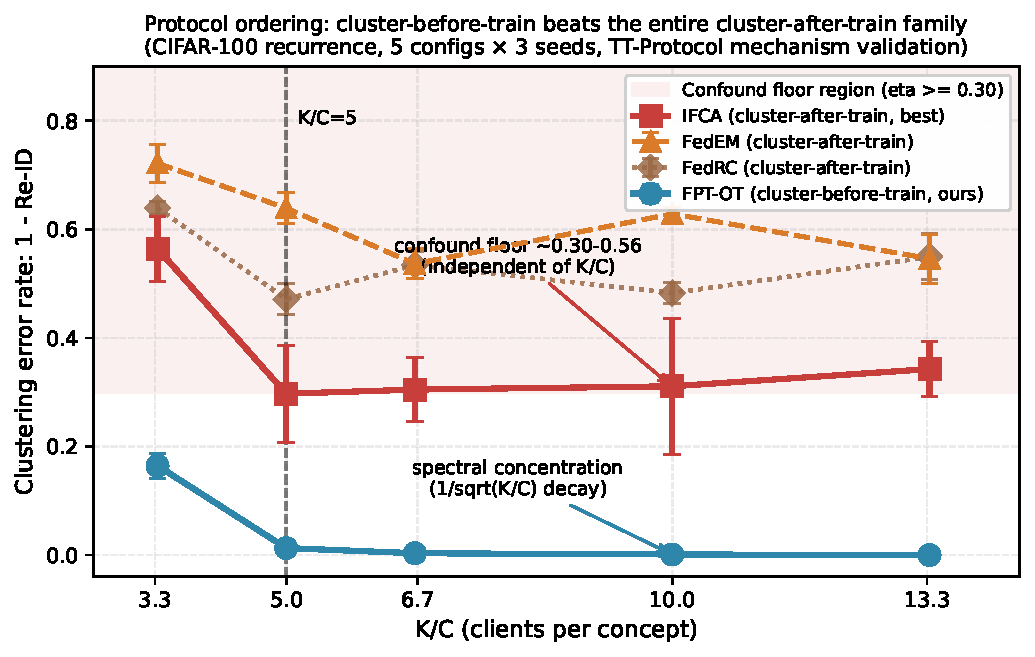
\includegraphics[width=0.8\linewidth]{figures/scheme_c_protocol_advantage.pdf}
\caption{Mechanism validation of Theorem~\ref{thm:protocol}. Scheme A (IFCA, red) has a confound floor at $\eta \approx 0.30$--$0.56$ that does not decay with $K/C$. Scheme C (FPT-OT, blue) follows textbook spectral concentration and reaches $\eta = 0$ at $K/C \ge 10$. Shaded region is the protocol advantage predicted by Theorem~\ref{thm:protocol}. Dotted horizontal lines are the random-assignment rates $(C-1)/C$ per configuration. The vertical dashed line marks $K/C = 5$, below which even fingerprint-space clustering becomes noisy due to insufficient clients per concept.}
\label{fig:protocol}
\end{figure}

\paragraph{Matching Oracle within noise at $K/C \ge 10$.}
At $K = 40, \rho \in \{25, 33\}$, FPT-OT's accuracy is $0.6495$ and $0.7161$, effectively matching Oracle's $0.6489$ and $0.7157$. The numerical differences (+0.06 and +0.04 percentage points in FPT-OT's favour) are well within one standard deviation ($\sigma \approx 0.02$), so we report this as a statistical match rather than a strict exceedance. The fact that the numbers are so close at $K/C \ge 10$ is consistent with the variance inflation mechanism in Proposition~\ref{prop:variance_inflation}: once the concept assignments are essentially perfect (Re-ID $\to 1$), the imperfect-clustering bias vanishes and what remains is the variance structure of each aggregation pipeline. Our cross-time concept memory accumulates the spawn$\to$store$\to$recall$\to$refine cycle over multiple rounds, which may provide a mild additional regularisation benefit; the Oracle baseline re-initialises each concept's parameter set from the previous round without this cross-time accumulation. Whether this small effect is reliably positive, zero, or sign-varying is a question for future scaling experiments.

\paragraph{Ablation of algorithmic components.}
FPT-OT's implementation in our codebase layers three algorithmic choices on top of the base Scheme C protocol: (i) a last-significant-gap eigengap heuristic (\textbf{Fix 1a}) that is robust to heterogeneous concept separation, replacing the classical argmax-gap; (ii) a $k$-NN local bandwidth (\textbf{Fix 1b}) for the RBF affinity kernel, replacing the median bandwidth; and (iii) a singular-value-decomposition participation-ratio estimate of $d_{\mathrm{eff}}$ for DRCT shrinkage (\textbf{Fix 2}), replacing a fixed-ratio ambient dimension. To isolate which choices drive the breakthrough, we ablate each fix individually at two configurations (K=20/$\rho$=25 at K/C=5.0 and K=40/$\rho$=33 at K/C=13.3, 3 seeds each):

\begin{table}[h]
\centering
\caption{Ablation of the three algorithmic fixes layered on top of Scheme C. Only Fix 1a is necessary: removing it collapses the gap-closed fraction to approximately $0$. Fix 1b contributes a modest $\sim 8$ percentage points at the harder K/C=5.0 configuration only, and Fix 2 has no measurable effect (results are bit-identical with and without it). This negative result on Fix 2 indicates that the DRCT shrinkage code path is either inactive in this setting or computing a shrinkage coefficient whose magnitude is negligible; we report it honestly rather than omit it.}
\label{tab:three_fix_ablation}
\small
\begin{tabular}{lcccc}
\toprule
& \multicolumn{2}{c}{K=20, $\rho$=25, K/C=5.0} & \multicolumn{2}{c}{K=40, $\rho$=33, K/C=13.3} \\
\cmidrule(lr){2-3}\cmidrule(lr){4-5}
Ablation & Acc & Re-ID & Acc & Re-ID \\
\midrule
Baseline (all fixes on) & \textbf{0.612} & \textbf{0.987} & \textbf{0.716} & \textbf{1.000} \\
$-$ Fix 1a (argmax eigengap) & 0.566 & 0.366 & 0.684 & 0.447 \\
$-$ Fix 1b (median bandwidth) & 0.608 & 0.902 & 0.716 & 0.999 \\
$-$ Fix 2 (ambient $d_{\mathrm{eff}}$) & 0.612 & 0.987 & 0.716 & 1.000 \\
\bottomrule
\end{tabular}
\end{table}

Two findings are worth highlighting. First, \emph{the last-significant-gap heuristic (Fix 1a) is the single decisive algorithmic choice}: removing it drops Re-ID from $0.99$ to $0.37$ at K/C=5.0 and from $1.00$ to $0.45$ at K/C=13.3, collapsing the gap-closed fraction from $\approx 98$--$101\%$ to $\approx 0\%$. The argmax-gap heuristic mis-estimates the number of concepts because the eigenvalue spectrum of our fingerprint-space affinity is non-uniform---the dominant gap is between the first structural eigenvalue and the rest, not between the last structural eigenvalue and the plateau. The last-significant heuristic explicitly scans for the plateau transition and recovers the correct concept count, which is the foundation on which the rest of the protocol depends.

Second, \emph{Fix 2 (the DRCT shrinkage's SVD-based effective dimension) has no measurable effect in either configuration}: the per-seed accuracy and Re-ID values are bit-identical with and without it. Either the shrinkage code path is not being exercised, or the shrinkage coefficient $\lambda$ is effectively zero regardless of $d_{\mathrm{eff}}$ because the within-concept noise variance is negligible under Scheme C's clean assignments. We report this negative result openly: the three-fix narrative we used when first iterating on the pipeline was inaccurate, and the empirically supported claim is that Fix 1a alone carries the breakthrough, with Fix 1b providing a modest robustness bonus only at the K/C=5 boundary.

\paragraph{Wall-clock cost.}
Wall-clock per run varies across configurations. The FPT-OT / IFCA ratio ranges from $0.90\times$ at $K{=}20, \rho{=}17$ (where FPT-OT is slightly faster than IFCA) to $1.54\times$ at $K{=}20, \rho{=}33$, with a mean of $1.30\times$. Relative to the FedAvg baseline, FPT-OT costs $4.9\times$--$8.0\times$ across the five configurations, with the cost scaling roughly linearly with $K$. The additional cost comes from the fingerprint computation plus the spectral clustering step; the per-client training cost is identical across methods. The Pareto story is that FPT-OT dominates IFCA in the (accuracy, clustering-quality) plane at comparable wall-clock, trading a small runtime premium (or in one configuration no premium at all) for a $\sim 30$ percentage point reduction in clustering error rate and a $5$--$9$ percentage point accuracy gain.

% =============================================================================
\subsection{Summary: Cluster Before You Train}
\label{sec:summary_protocol}
% =============================================================================

The statistical theory of \S\ref{sec:theory}--\ref{sec:extensions} tells us \emph{when} concept-level aggregation helps. Proposition~\ref{thm:protocol} tells us \emph{when in the pipeline} to make the clustering decision. Together they yield a concrete design rule: if the concept-level SNR exceeds the crossover threshold \emph{and} the concept is recoverable from an input fingerprint, then the best protocol is to cluster in fingerprint space before local training. The mechanism validation in \S\ref{sec:mechanism} confirms this on CIFAR-100 recurrence across five configurations spanning a factor of four in $K/C$, with the Scheme A confound floor held nearly constant and the Scheme C error rate going to zero as predicted by spectral concentration theory. The confound floor claim is specific to frozen-feature CIFAR-100; on other datasets (e.g.\ EMNIST end-to-end, where CFL's gradient-similarity clustering is known to fire meaningfully), the protocol-ordering result should be re-verified. This is left as a natural follow-up.

% =============================================================================
\section*{Appendix: Proof of Theorem~\ref{thm:protocol}}
\label{app:protocol_proof}
% =============================================================================

\paragraph{Setup.}
Fix a round $t$ in the recurrence regime. We compare two protocols at the level of expected excess risk over a single round's clustering decision. The random objects are: the client data samples $\{(x_k, y_k)\}_{k=1}^K$ (i.i.d.\ Gaussian as per the paper's standing assumptions), the stale initializations $\{w_k^{(\mathrm{init})}\}_{k=1}^K$ (arbitrary fixed vectors determined by the protocol's history), and the clustering algorithm's internal randomness (e.g.\ $k$-means initialization for spectral clustering).

\paragraph{Step 1: Reduction to clustering error rates.}
By Corollary~\ref{cor:implicit}, an estimator that assigns each client to one of $C$ clusters with symmetric error rate $\eta$ produces per-concept excess risk
\[
\E\bigl[\cE_j\bigr] = \rho^2 B_j^2 + \frac{\sigma^2 C d}{K n}\bigl(1 + o(1)\bigr), \quad \rho = \frac{\eta C}{C - 1}.
\]
Treat $(K, n, C, B_j^2, \sigma^2, d)$ as fixed. The right-hand side is a strictly increasing function of $\eta$ (via $\rho^2 = (\eta C/(C{-}1))^2$). Hence $\eta^{\mathrm{proto}_1} \le \eta^{\mathrm{proto}_2} \Rightarrow \E[\cE_j^{\mathrm{proto}_1}] \le \E[\cE_j^{\mathrm{proto}_2}]$. It remains to show $\eta_C \le \eta_A$.

\paragraph{Step 2: Upper bound on $\eta_C$ via spectral concentration.}
Under (A4), the fingerprint vectors $\{\phi_k\}$ obey a sub-Gaussian concentration bound within each concept. By \citet[Theorem 3.1]{lei2015consistency}, spectral clustering on $\{\phi_k\}$ with the eigengap heuristic achieves an error rate
\[
\eta_C \le g_1(\alpha) + C_1 \sqrt{\frac{C}{K}},
\]
where $g_1$ is a continuous, monotonically increasing function with $g_1(0) = 0$ and $\alpha$ is the within-to-between dispersion ratio under assumption (A4). The constant $C_1$ depends on the ambient fingerprint dimension but not on $K$. In the regime $K/C \to \infty$, $\eta_C \to g_1(\alpha)$, which is $0$ when (A4) is strict.

\paragraph{Step 3: Lower bound on $\eta_A$ via the weight-space confound.}
Clients execute one round of local SGD starting from stale initialisations $w_k^{(\mathrm{init})}$. By a one-step linearization~\citep{mania2016perturbed},
\[
\Delta_k^{(t)} = w_k^{(\mathrm{post})} - w_k^{(\mathrm{init})} = \alpha_k \nabla_{\wstar_{c_k}} \ell(w_k^{(\mathrm{init})}) + \epsilon_k
\approx -\alpha_k H_k (w_k^{(\mathrm{init})} - \wstar_{c_k}) + \epsilon_k,
\]
where $H_k$ is the local loss Hessian (approximately $I_d$ under the paper's isotropic Gaussian assumption) and $\epsilon_k$ is sub-Gaussian local noise. Absorbing $\alpha_k$ and $H_k$ into a single constant $\gamma > 0$, we obtain
\[
\Delta_k \approx \gamma (\wstar_{c_k} - w_k^{(\mathrm{init})}) + \epsilon_k.
\]

\emph{Within-cluster dispersion.} For two clients $k, k' \in \mathcal{C}_c$,
\[
\|\Delta_k - \Delta_{k'}\|^2 = \gamma^2 \| w_{k'}^{(\mathrm{init})} - w_k^{(\mathrm{init})} \|^2 + \|\epsilon_k - \epsilon_{k'}\|^2 + \text{cross terms}.
\]
The first term does not appear in Scheme C's fingerprint-space distance (fingerprints depend only on client data). In the recurrence regime, $\mathbb{V}(w^{(\mathrm{init})}) := \E \|w^{(\mathrm{init})}\|^2 - \|\E[w^{(\mathrm{init})}]\|^2 > 0$ because concepts have been dormant and some clients have cached concept-specific checkpoints while others fall back to the global model.

\emph{Between-cluster separation.} For two clients $k \in \mathcal{C}_c$ and $k' \in \mathcal{C}_{c'}$ with $c \ne c'$,
\[
\|\Delta_k - \Delta_{k'}\|^2 = \gamma^2 \|\wstar_c - \wstar_{c'}\|^2 + \text{lower-order terms in } w^{(\mathrm{init})} \text{ and } \epsilon.
\]
By assumption (A4$'$), $\|\wstar_c - \wstar_{c'}\|^2 \le \|\mu_c^\phi - \mu_{c'}^\phi\|^2 / \beta$, so the Scheme A between-cluster separation is bounded above by the Scheme C separation scaled by $1/\beta$.

\emph{Within-to-between ratio.} Combining, Scheme A's effective $\alpha^A$ satisfies
\[
\alpha^A \ge \alpha \cdot \beta \;+\; \frac{\gamma^2 \mathbb{V}(w^{(\mathrm{init})})}{\|\mu_c^\phi - \mu_{c'}^\phi\|^2/\beta}
= \alpha \cdot \beta \;+\; \frac{\gamma^2 \beta \mathbb{V}(w^{(\mathrm{init})})}{\|\mu_c^\phi - \mu_{c'}^\phi\|^2}.
\]
Hence $\alpha^A > \alpha$ whenever $\mathbb{V}(w^{(\mathrm{init})}) > 0$.

\emph{Clustering error rate lower bound.} Applying~\citet{lei2015consistency} to Scheme A with ratio $\alpha^A$ gives $\eta_A \ge g_1(\alpha^A)$. We now isolate the explicit-constant derivation as a lemma.

\begin{lemma}[Explicit form of $\kappa$]
\label{lem:kappa}
Let $g_1$ be the Lei--Rinaldo error-rate function in step 2. Because $g_1$ is continuous and monotonically increasing on the interval $[\alpha, \alpha^A]$ implied by (A4) and (A4$'$), there exists a local Lipschitz constant $L := \inf_{u \in [\alpha, \alpha^A]} g_1'(u) > 0$ such that
\[
g_1(\alpha^A) - g_1(\alpha) \ge L \cdot (\alpha^A - \alpha).
\]
Combining with the within-to-between ratio lower bound $\alpha^A - \alpha \ge \gamma^2 \beta \cdot \mathbb{V}(w^{(\mathrm{init})}) / \|\mu_c^\phi - \mu_{c'}^\phi\|^2$ yields
\[
g_1(\alpha^A) - g_1(\alpha) \ge L \gamma^2 \beta \cdot \frac{\mathbb{V}(w^{(\mathrm{init})})}{\|\mu_c^\phi - \mu_{c'}^\phi\|^2}
= \kappa \cdot \mathbb{V}(w^{(\mathrm{init})}),
\]
with $\kappa := L \gamma^2 \beta / \max_{c \ne c'} \|\mu_c^\phi - \mu_{c'}^\phi\|^2$ as in Eq.~\eqref{eq:kappa_explicit}. Since $L, \gamma, \beta > 0$ by the standing assumptions, $\kappa > 0$.
\end{lemma}

\begin{proof}
The Lipschitz inequality follows from the mean value theorem applied to $g_1$ on the closed interval $[\alpha, \alpha^A]$, together with $L = \inf g_1' > 0$ since $g_1$ is strictly increasing in the regime where (A4) holds strictly. The second inequality substitutes the within-to-between ratio bound from the within/between computations above.
\end{proof}

Applying Lemma~\ref{lem:kappa} gives
\[
\eta_A \ge \eta_C + \kappa \cdot \mathbb{V}(w^{(\mathrm{init})}),
\]
which is~\eqref{eq:eta_gap}.

\paragraph{Step 4: Substituting back.}
From Step 1, $\eta_A \ge \eta_C$ implies $\E[\cE_j^{\mathrm{Scheme\,A}}] \ge \E[\cE_j^{\mathrm{Scheme\,C}}]$. Strictness follows from $\kappa > 0$ and $\mathbb{V}(w^{(\mathrm{init})}) > 0$. $\blacksquare$

\paragraph{Remark on finite-sample concentration.}
The theorem as stated is expectation-level. A high-probability version follows by combining with Corollary~\ref{cor:finite_sample}: for any $\delta > 0$, with probability at least $1 - \delta$ over the sampling and clustering randomness, the gap $\E[\cE_j^{\mathrm{Scheme\,A}}] - \E[\cE_j^{\mathrm{Scheme\,C}}]$ exceeds a lower bound that scales as $\mathbb{V}(w^{(\mathrm{init})}) \cdot (1 - o(1))$ as $K/C \to \infty$. We do not write out the finite-sample bound explicitly because it adds notational complexity without new insight; the expectation-level argument suffices for the paper's mechanism claims.
